\graphicspath{{figs/Chp-FGaBP/}}


%%Fakesection Acronym reset
\glsreset{acr:fg}
\glsreset{acr:gm}
\glsreset{acr:bp}
\glsreset{acr:fgabp}
\glsreset{acr:femfg}
\glsreset{acr:ca}
\glsreset{acr:aufgabp}
\glsreset{acr:mgpcg}
\glsreset{acr:pwgabp}
\glsreset{acr:pwgm}
\glsreset{acr:spd}
\glsreset{acr:csr}
\glsreset{acr:dpcg}
\glsreset{acr:nmr}
\glsreset{acr:emr}
\glsreset{acr:su}
\glsreset{acr:ssc}

\chapter{Parallel Solution of the Finite Element Method Using Gaussian Belief Propagation}
\label{chp:FGaBP}

%%Fakesection From abstract
The proliferation of parallel architectures such as manycore CPUs and GPUs drives the need to redesign conventional algorithms with parallelism in mind.
However, the parallel performance of conventional \gls{acr:fem} implementations can be limited by the inherent coupling of the underlying sparse data-structures.
In this chapter, we look into \gls{acr:bp} inference algorithms to address these challenges.
We introduce a probabilistic \gls{acr:gm} of the \gls{acr:fem} based on \glspl{acr:fg} by recasting the global deterministic \gls{acr:fem} as a localized variational inference problem.
The resulting algorithm eliminates the need to assemble any global sparse data-structure or perform any global sparse algebraic operation.


\section{Introduction}
\label{sec:gabpIntro}
%From Introduction section
We have presented in \secRef{sec:pwgabp} a background of the \gls{acr:pwgabp} algorithm and showed that it is a recursive message passing algorithm that offers distributed computations \cite{bib:Pearl88ProbabilisticReasoning, bib:Weiss01CorrectnessBelief, bib:Shental2008GBPSSLE}.
\gls{acr:pwgabp} demonstrated better empirical results than conventional iterative solvers such as Jacobbi, \gls{acr:gs}, \gls{acr:sor} and \gls{acr:dpcg} for \gls{acr:sdd} matrices \cite{bib:El-Kurdi2012EIOGBPSFLSDDLS, bib:Shental2008GBPSSLE, bib:El-Kurdi2012RGBP}.
We have also shown in \chpRef{chp:PW-GaBP} that the \gls{acr:pwgabp} algorithm can potentially parallelize \gls{acr:fem} applications when using scheduling schemes that facilitates its parallel execution \cite{bib:El-Kurdi2012RGBP}.
While new schemes were introduced in \chpRef{chp:relGaBP} to accelerate the \gls{acr:pwgabp} for \gls{acr:fem} matrices using the dynamic relaxation \gls{acr:drgabp} algorithm, the overall performance of the \gls{acr:drgabp} algorithm was still short of popular solvers such as the \gls{acr:icpcg} solver.
However, the \gls{acr:pwgabp} solver, and similarly all other conventional solvers, still requires the assembly of a large sparse matrix data-structure.
Many applications that require repeated reassembly of the global matrix, such as adaptive multigrid and non-linear applications, can suffer from the long setup time of the sparse matrix.


We believe that the assembly of the sparse matrix and the algebraic operations on such data-structures are the sources of bottlenecks that are hindering efficient parallel implementations for the \gls{acr:fem} computation on \gls{acr:hpc} platforms.
Novel and inherently parallel algorithms, therefore, need to be developed from a completely different perspective in order to address this issue.
The classical variational formulation of the \gls{acr:fem} provides useful physical insight for the underlying \gls{acr:bvp}, which leads us to exploring the use of a different breed of algorithms used in variational inference such as \gls{acr:bp} \cite{bib:Pearl88ProbabilisticReasoning}.
In this work, we present a new \gls{acr:bp}-based algorithm specifically derived for the \gls{acr:fem} that is referred to as the \gls{acr:fgabp}.
We first develop a variational inference formulation for the \gls{acr:fem} in order to facilitate its interpretation as a \gls{acr:gm} problem.
We then introduce the \gls{acr:fg} model for the variational inference \gls{acr:fem} referred to as the \gls{acr:femfg} model.
Next, we use the new \gls{acr:femfg} model to develop the \gls{acr:fgabp} algorithm.
We show that the \gls{acr:fgabp} algorithm is applicable for arbitrary element geometry and interpolation order, which is needed to address a wide variety of \gls{acr:fem} applications.
The \gls{acr:fgabp} algorithm provides better parallel computations than conventional algebraic methods by avoiding the assembly of the global sparse matrix, and by solving the \gls{acr:fem} in parallel element-by-element without the need to perform any global sparse matrix operations.
The new algorithm provides flexible memory bandwidth utilization due to its use of distributed message-based computations, referred to as message scheduling, which allows us to adapt its implementation on hardware using various memory architectures without impacting the algorithm's computational stability.
Such a critical advantage is usually lost when adapting reformulation techniques of the \gls{acr:cg} solver such as the \gls{acr:ca} \cite[p. 34]{bib:Hoemmen2010EECS} which is based on the $s$-step \cite{bib:Chronopoulos1989153} method.




The chapter is organized as follows.
In \secRef{sec:FEMVI} we present the formulation of the \gls{acr:fem} as a variational inference problem.
In \secRef{sec:FEMFG} we introduce the \gls{acr:femfg} model, and in \secRef{sec:femgabp} we derive \gls{acr:bp} update rules on the \gls{acr:femfg} and present the \gls{acr:fgabp} algorithm.
In \secRef{sec:lowerCompFGaBP} we present reformulations of the \gls{acr:fgabp} algorithm that considerably reduce its computational complexity.
In \secRef{sec:elmMerg} we present the element merge solution that enhances the memory bandwidth utilization of the \gls{acr:fgabp} algorithm.
In \secRef{sec:fgabpImp} we detail implementation analysis for the \gls{acr:fgabp} algorithm.
Finally, in \secRef{sec:fgabpRes} we conclude with our results and discussions illustrating the \gls{acr:fgabp} execution on \gls{acr:fem} problems.


\section{The FEM as a Variational Inference Problem}
\label{sec:FEMVI}


The work in \cite{bib:Yedidia2004CFEAAGBPA,bib:Yedidia2000genbp}, introduced by Yedidia et al., shows that the \gls{acr:bp} solution on \gls{acr:fg} models corresponds to the Bethe approximation of the free energy \cite{bib:Bethe,bib:Kikuchi} associated with the underlying inference model.
Using that insight, we will derive the \gls{acr:fgabp} algorithm to minimize the variational energy of the \gls{acr:fem} problem.
To that end, we first model the \gls{acr:fem} in terms of a probabilistic \gls{acr:gm} referred to as the \gls{acr:fem} Factor Graph (\gls{acr:femfg}).
We start by reformulating the \gls{acr:fem} as a variational inference problem by modifying the \gls{acr:fem} functional \eqnRef{eqn:discFunc} as follows:

\begin{align}
	\mathcal{P}(U) & = \frac{1}{Z} \exp\left[ -  \sum_{s\in\mathcal{S}}\mathcal{F}_s(U_s) \right] \label{eqn:gpf}\\
	& = \frac{1}{Z} \prod_{s \in \mathcal{S}} \Psi_s(U_s) \label{eqn:fgpf}
\end{align}
where $Z$ is a normalizing constant and $\Psi_s(U_s)$ are local factor functions of the local finite element variables $U_s$ defined as:
\begin{equation}
	\Psi_s(U_s) = \exp\left[ -\frac{1}{2} U^T_s M_s U_s +B_s^T U_s\right]. \label{eqn:Psi}
\end{equation}
It is worth noting that $\Psi_s$ as defined in (\ref{eqn:Psi}) takes a multivariate Gaussian form albeit unnormalized when the element characteristic matrix $M_s$ is \gls{acr:spd}.
\appRef{app:gaDiss} presents more details about Gaussian distributions and their properties.

It can be shown that $\mathcal{P}$ as in (\ref{eqn:gpf}) represents a Gaussian multivariate probability distribution when $\mathcal{F}$ is convex quadratic \cite{bib:Wainwright2008GMEFAVI}.  Hence, the optimality condition of $\mathcal{F}$ can be restated as:
\begin{equation}
	\argmin_{U} \mathcal{F} = \argmax_{U} \mathcal{P}. \label{eqn:statPoint}
\end{equation}
Here, we assume that the variables vector $U$ will represent joint Gaussian random variables under the distribution $\mathcal{P}$.
Since $\mathcal{P}$ is maximized when $U = \mu$, where $\mu$ is the mean vector of $\mathcal{P}$, the \gls{acr:fem} minimization problem of the functional $\mathcal{F}$ is transformed into a computational inference problem of finding the marginal means of the random variables $U$ under the distribution $\mathcal{P}$.
Hence, \gls{acr:bp} inference algorithms can be employed to compute the marginal means of the random variables $U$.

Now, we turn our attention to the normalizing constant $Z$ in \eqnRef{eqn:gpf}.
Wainright and Jordan have presented a framework for variational inference on exponential distributions in \cite{bib:Wainwright2008GMEFAVI}.
We will follow a similar approach to analyze the distribution $\mathcal{P}$.
In our case, $Z$ ensures that $\mathcal{P}$ is a valid distribution such that:
\begin{equation}
	\int_U \mathcal{P}\, \mathrm{d} U = 1
\end{equation}
or alternatively:
\begin{equation}
	Z(M_s,B_s) = \int_U \exp \left( \mathcal{-F} \right)\, \mathrm{d} U <+\infty,\,\,\,\forall s
\end{equation}
that is $Z$ is a function of $M_s$ and $B_s$ such that $Z(M_s,B_s)$ is finite.
Since $\mathcal{F}$ is quadratic, and by convex analysis, finiteness of the integral can be met by ensuring that the element matrices $M_s$ are positive definite.
Observing that $\mathcal{F}$ can also be represented in an assembled form, then the finiteness requirement can alternatively be met by ensuring that the assembled form of the \gls{acr:fem} matrix is positive definite.
Note that the symmetry condition on $M_s$ can be imposed only to simplify the \gls{acr:bp} update rules derivations by assuming Gaussian distributions for the underlying random variables, as will be shown in the following sections.


\section{The FEM Factor Graph Model}
\label{sec:FEMFG}

Given the distribution $\mathcal{P}(U)$, one can define a \gls{acr:gm} to perform computational inference in order to infer the marginal distributions of the random variables in $U$.
A widely used class of \glspl{acr:gm} is the \gls{acr:fg} ~\cite{bib:Kschischang2001FGATSA}, which is a bipartite \gls{acr:gm} that directly represents the factorization of $\mathcal{P}$.
We refer to the \gls{acr:fg} model derived from the distribution $\mathcal{P}$ as the \gls{acr:femfg} model.
The \gls{acr:femfg}, as shown in \figRef{fig:FEM_FG}, includes two types of nodes, a random variable node ($u_i$) representing each node in the unknown vector $U$, and a factor node representing the local factors $\Psi_s$.
An edge is inserted between a variable node $u_i$ and a factor node $\Psi_s$ if $u_i$ is an argument of the local factor $\Psi_s$.
For example, the two element \gls{acr:fem} shown in \figRef{fig:FEM_mesh} can be represented by the probability functional $\mathcal{P}(U)=\Psi_a(u_1,u_2,u_3,u_4,u_5,u_6)\Psi(u_4,u_5,u_6,u_7,u_8,u_9)$.  Likewise, the \gls{acr:femfg} shown in \figRef{fig:FEM_FG} contains two factor nodes labeled \fn{a} and \fn{b} each for $\Psi_a$ and $\Psi_b$ correspondingly.
The node \fn{a} has edges to the variable nodes set $\{u_1,u_2,u_3,u_4,u_5,u_6\}$ that are arguments of $\Psi_a$ and, similarly, the node \fn{b} is connected to variable nodes that are arguments of $\Psi_b$.


The \gls{acr:pwgm}, corresponding to the same mesh, is also provided in \figRef{fig:FEM_PW} for comparison.
As mentioned in \secRef{sec:pwgabp}, the \gls{acr:pwgm} model is used to derive the \gls{acr:pwgabp} algorithm as a solver for linear systems of equations \cite{bib:Shental2008GBPSSLE}.
From that perspective, it may seem that the \gls{acr:pwgabp} algorithm has a greater degree of generality; however, the \gls{acr:pwgabp} has major shortcomings when used for \gls{acr:fem} problems.
Mainly, the \gls{acr:pwgm} does not benefit from the underlying \gls{acr:fem} problem structure; as a result, the number of communication links in the \gls{acr:pwgm} is much higher in comparison to the \gls{acr:femfg} model for certain meshes.
While it may be easy to deduce the structure of the \gls{acr:femfg} model from the underlying \gls{acr:fem} mesh, it is important to note that the number of vertices or edges in a mesh does not necessarily correspond to the number of vertices or edges in a \gls{acr:femfg} model as shown in \figRef{fig:FEM_PW}.
We can illustrate the link reduction advantage of the \gls{acr:femfg} model by counting the links in the same example diagrams.
From the figures, the \gls{acr:femfg} requires 12 links while the \gls{acr:pwgm} requires 27 links for a mesh of two second order triangles.
Similarly, link reductions can also be illustrated considering first order quadrilateral and hexahedral meshes and second order tetrahedral meshes.
In fact, the reduction in the number of links for the \gls{acr:femfg} model progressively increases with the order of the \gls{acr:fem} element.
More detailed analysis on this will be provided later in \secRef{sec:fgabpImp}, where we discuss the implementation details.
First order triangular and tetrahedral meshes are the only case where the \gls{acr:femfg} model will contain more links than the \gls{acr:pwgm}.
To remedy this situation, we provide a solution that lowers the number of links in the \gls{acr:femfg} model for first order triangular and tetrahedral meshes by merging elements that share edges or faces.
The element merging solution is detailed in \secRef{sec:elmMerg}.

\begin{figure}[t]
	\centering{
	\subfloat[]{
	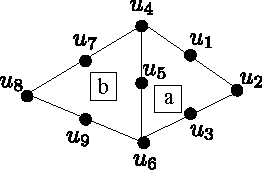
\includegraphics[scale=1.0]{FEM_mesh} \label{fig:FEM_mesh}
	}
  %\hspace{+1mm}
	\subfloat[]{
	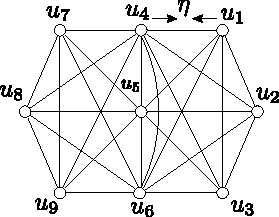
\includegraphics[scale=0.95]{FEM_PW} \label{fig:FEM_PW}
	}
  %\hspace{+2mm}
	\subfloat[]{
	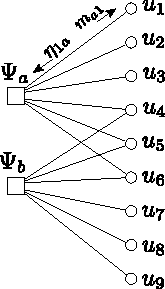
\includegraphics[scale=1.0]{FEM_FG} \label{fig:FEM_FG}
	}
	}
	\caption[Sample \acrshort{acr:femfg}.]{\protect\subref*{fig:FEM_mesh} Sample \gls{acr:fem} mesh of two second order triangles.  Two \gls{acr:gm} representations are shown in \protect\subref*{fig:FEM_PW} and \protect\subref*{fig:FEM_FG}; the messages $\eta$ in a \gls{acr:gm} are communicated recursively either sequentially or in parallel. ~\protect\subref*{fig:FEM_PW}~The conventional \glspl{acr:pwgm}. \protect\subref*{fig:FEM_FG}~The new \gls{acr:femfg} model with reduced number of communication links and improved parallelism.}
	\label{fig:FEM_GM}
\end{figure}



An important remark to make on the \gls{acr:fem} distribution $\mathcal{P}$ is that it is conveniently represented in a factorized form due to its direct derivation from the \gls{acr:fem} functional \eqnRef{eqn:discFunc}.
This factorization reflects the structure of the underlying \gls{acr:fem} mesh that is used to derive the \gls{acr:femfg} model.
In fact, the local factor functions $\Psi_s$ are functions over the cliques in the \gls{acr:pwgm} model representing the sparse matrix we would have obtained, if we chose to assemble the \gls{acr:fem} linear system of equations.
Nonetheless, the term clique is used here for technical convenience since, due to the factorized nature of the exponential distribution $\mathcal{P}$, higher orders of cliques can be formed in the \gls{acr:femfg} model by introducing zero edges in order to form other supersets of cliques.
This can be used, for instance, to improve the memory bandwidth utilization of the algorithm for certain triangular or tetrahedral meshes as later discussed in \secRef{sec:elmMerg}.
This indicates that the \gls{acr:femfg} representation is more adept in exploiting the \gls{acr:fem} problem structure than the \gls{acr:pwgm} representation used for the \gls{acr:pwgabp} solver.
In addition to this flexibility, the \gls{acr:fgabp} algorithm, based on the \gls{acr:femfg} model, demonstrates improved convergence versus the \gls{acr:pwgabp}, as shown later in \secRef{sec:fgabpRes}.
We believe that this improved convergence is a direct consequence of the \gls{acr:femfg} model better exploiting the underlying \gls{acr:fem} problem's structure.
In addition, inference on \gls{acr:femfg} can perform more dense and localized computations (correlating more of the local variables states) resulting in less communication as opposed to inference on \glspl{acr:pwgm}.


Lastly and most importantly, the \gls{acr:pwgabp}, as well as other conventional iterative solvers still require the assembly of the large sparse matrix $A$ while the \gls{acr:femfg} model eliminates this costly step.
Another key advantage of using the \gls{acr:femfg} model as opposed to the \gls{acr:pwgm} is that the \gls{acr:femfg} configuration draws naturally from the \gls{acr:fem} mesh.
To illustrate this advantage, we consider the hypothetical scenario where one would attempt to generate an \gls{acr:femfg} (or maximal clique \gls{acr:fg} configuration) from a \gls{acr:pwgm}.
Clearly, considerable overhead processing is needed in order to use specialized algorithms, such in \cite{bib:BronK1973,bib:TomitaTT2006,bib:Akkoyunlu1973,bib:Szabo2011,bib:Darehmiraki2009}, to identify the maximal cliques in the \gls{acr:pwgm}.
In addition to identifying cliques, one would still need to perform the proper edge coefficient splitting on edges shared between cliques while maintaining the numerical integrity of the \gls{acr:bp} inference algorithm.
A task that may prove difficult for ill-conditioned systems.

\section{The FGaBP Algorithm}
\label{sec:femgabp}

To derive the update rules of the \gls{acr:fgabp} algorithm, two levels of specialization need to be applied to the general \gls{acr:bp} rules introduced previously in \secRef{sec:bp}.
First, we setup the \gls{acr:bp} inference algorithm on the new \gls{acr:femfg} model of the introduced \gls{acr:fem} variational inference functional \eqnRef{eqn:gpf}.
Then, recognizing that the \gls{acr:fem} inference functional \eqnRef{eqn:gpf} takes a Gaussian form; as a result, all the update messages will take a Gaussian form.
Hence, the multidimensional integral in (\ref{eqn:genFNUM}) can be solved in a closed form which reduces the update messages to propagating only the Gaussian parameters.


\subsection{The FGaBP Update Rules}

In this section we detail all the \gls{acr:bp} update rules formulation for the \gls{acr:fgabp} algorithm.


\subsubsection{Gaussian Parameterization}

For our development of the \gls{acr:fgabp}, we use a specific Gaussian distribution parametrization referred as the canonical parameterization, or the information form.
More details on this parameterization and its relationship to the normal Gaussian distribution form is provided in \appRef{app:gaDiss}.
The univariate canonical Gaussian form is defined as:
\begin{equation}
	G(\alpha,\beta)\propto\exp\left[\frac{-1}{2}\alpha u^2+\beta u\right]
\end{equation}
where $\alpha$ is the first canonical parameter that is equivalent to the reciprocal of the Gaussian variance; and $\beta$ is the second parameter.
For multivariate Gaussian distributions, we use the following parameterized form:
\begin{equation}
	\mathcal{G}(W,K)\propto\exp\left[\frac{-1}{2}U^TWU+K^T U\right]
\end{equation}
where $U$ is a vector of random Gaussian unknowns of arbitrary dimension, e.g. $n$; $W$ is the first canonical parameter which is an $n\text{-by-}n$ matrix assumed to be \gls{acr:spd}; $K$ is the second parameter which is a vector of the same dimension $n$.
We use proportionality in the Gaussian distributions because we do not require any normalization.
In general, the normalization constant is used to generate valid probability distributions such that the area underneath the distribution is equal to one.
Since in our setting we are only interested in the parameters of the distribution, $\alpha$ and $\beta$, rather than the distribution itself, which are sufficient to identify all the messages' distributions in the \gls{acr:fgabp} algorithm without the need of any normalization.


We start by making the assumption that the random variables $u_i \in U$ take Gaussian distributions as follows:
\begin{equation}
	u_i  \sim G(\alpha_i,\beta_i) \label{eqn:vndis}.
\end{equation}
As a result, the \gls{acr:bp} messages $m_{ai}$ and $\eta_{ia}$, as in \eqnRef{eqn:genFNUM} and \eqnRef{eqn:genVNUM}, take Gaussian forms parametrized by $\alpha$ and $\beta$.
This follows from the properties of multiplication and marginalization of Gaussian distributions as detailed in \appRef{app:gaDiss}.
Therefore substituting the \gls{acr:fem} local element function $\Psi_a$ \eqnRef{eqn:Psi} into \eqnRef{eqn:genFNUM}, the \gls{acr:bp} update rules in \eqnRef{eqn:genFNUM}, \eqnRef{eqn:genVNUM}, and \eqnRef{eqn:genB} can be reduced to propagating parameters $\alpha$ and $\beta$ between factor and variable nodes in the \gls{acr:femfg} graph.



\subsubsection{Variable Node Updates}


For each Variable Node $i$ (\vn{i}) process, compute the outgoing messages ($\alpha_{ia}, \beta_{ia}$) to each Factor Node $a$ (\fn{a}), such that $a\in \neih{i}$, as follows:
\begin{align}
	\alpha_{ia}^{(t)} & = \sum_{k\in\mathcal{N}(i)\setminus a}\alpha_{ki}^{(t_\star)} \label{eqn:vnaSumMin}\\
	\beta_{ia}^{(t)} & =\sum_{k\in\mathcal{N}(i)\setminus a}\beta_{ki}^{(t_\star)}. \label{eqn:vnbSumMin}
\end{align}
where $t$ and $t_\star$ are iteration counts such that $t_\star \leq t$.
However, this computational complexity can be reduced considerably if we compute the \gls{acr:vn} messages in two stages.
In the first stage, combine all incoming messages ($\alpha_{ai}, \beta_{ai}$) from each \fn{a}, $a\in \neih{i}$, into the nodal parameters ($\alpha_i, \beta_i$) as follows:
\begin{align}
	\alpha_{i}^{(t_\star)} & = \sum_{k\in\mathcal{N}(i)}\alpha_{ki}^{(t_\star)} \label{eqn:vnaSum}\\
	\beta_{i}^{(t_\star)} & =\sum_{k\in\mathcal{N}(i)}\beta_{ki}^{(t_\star)}. \label{eqn:vnbSum}
\end{align}
Then in the second stage, compute the outgoing messages ($\alpha_{ia}, \beta_{ia}$) to each \fn{a} as follows:
\begin{align}
	\alpha_{ia}^{(t)} & =\alpha_{i}^{(t_\star)}-\alpha_{ai}^{(t_\star)} \label{eqn:vna}\\
	\beta_{ia}^{(t)} & =\beta_{i}^{(t_\star)}-\beta_{ai}^{(t_\star)}. \label{eqn:vnb}
\end{align}
It is important to maintain the \gls{acr:bp} message consistency when using the second approach.
The \gls{acr:bp} message consistency is maintained here when the same $t_\star$ value on each individual link is used for all equations in \eqnRef{eqn:vnaSum}, \eqnRef{eqn:vna}, \eqnRef{eqn:vnbSum}, and \eqnRef{eqn:vnb}.  
Using this approach, the complexity of a \gls{acr:vn} message computation is reduced from $\bigo{2m(m-1)}$ to $\bigo{4m}$ for $m>3$, where $m$ is the number of the \gls{acr:vn} edges.


\subsubsection{Factor Node Updates}


For each \fn{a} process:
\begin{enumerate}
	\item Receive messages $(\alpha_{ia}^{(t_\star)}, \beta_{ia}^{(t_\star)})$, where $i\in\mathcal{N}(a)$.
	\item Define $\mathcal{A}^{(t_\star)}$ and $\mathcal{B}^{(t_\star)}$ such that $\mathcal{A}^{(t_\star)}$ is a diagonal matrix of incoming $\alpha_{ia}^{(t_\star)}$ parameters, and $\mathcal{B}^{(t_\star)}$ is a vector of incoming $\beta_{ia}^{(t_\star)}$ parameters as follows:
		\begin{equation}
			\begin{array}{cc}
				\mathcal{A}_a^{(t_\star)} =\left[\begin{array}{cccc}
					\alpha_{i_1a}^{(t_\star)} & 0 & \cdots & 0\\
					0 & \alpha_{i_2a}^{(t_\star)} & \cdots & 0\\
					\vdots & \vdots & \ddots & \vdots\\
					0 & 0 & \cdots & \alpha_{i_na}^{(t_\star)}
				\end{array}\right],
				& 
				\mathcal{B}_a^{(t_\star)} =\left[\begin{array}{c}
					\beta_{i_1a}^{(t_\star)}\\
					\beta_{i_2a}^{(t_\star)}\\
					\vdots\\
					\beta_{i_na}^{(t_\star)}
				\end{array}\right],
			\end{array}
			\label{eqn:fWK}
		\end{equation}
		where $\{ i_1, i_2, \dots, i_n \} = \mathcal{N}(a)$.
		Then, compute $W$ and $K$ as follows:
		\begin{align}
			W^{(t_\star)} &=M +\mathcal{A}^{(t_\star)}\\
			K^{(t_\star)} &=B +\mathcal{B}^{(t_\star)}
		\end{align}
		where  $M$ and $B$ are the element $a$ characteristic matrix and source vector as defined in \eqnRef{eqn:Psi} with $s=a$. 
	\item Partition $W^{(t_\star)}$ and $K^{(t_\star)}$ as follows:
		\begin{equation}
			\begin{array}{cc}
				\begin{aligned}
					W^{(t_\star)} & =\left[
					\begin{array}{cc}
						W^{(t_\star)}_{d,d} & V^{T}\\
						V & \bar{W}^{(t_\star)}
					\end{array}
					\right],
				\end{aligned} &
				\begin{aligned}K^{(t_\star)} &
					=\left[\begin{array}{c}
						K^{(t_\star)}_{d}\\
						\bar{K}^{(t_\star)}
					\end{array}\right]
				\end{aligned}
			\end{array}
			\label{eqn:wk}
		\end{equation}
		where $d = \mathcal{L}(i)$ is the local index corresponding to the global variable node $i$.
	\item Compute and send \fn{a} messages ($\alpha_{ai}^{(t)}$,~$\beta_{ai}^{(t)}$) to each \vn{i}, $i \in \neih{a}$, as follows:
		\begin{align}
			\alpha_{ai}^{(t)} & =M_{d,d}-V^{T}(\bar{W}^{(t_\star)})^{-1}V \label{eqn:fnaO}\\
			\beta_{ai}^{(t)} & =B_{d}-(\bar{K}^{(t_\star)})^{T}(\bar{W}^{(t_\star)})^{-1}V. \label{eqn:fnbO}
		\end{align}
\end{enumerate}


Note that the incoming messages $(\alpha_{ia},\beta_{ia})$ have been subtracted from \eqnRef{eqn:fnaO} and \eqnRef{eqn:fnbO}.  Also, it is worth mentioning that the arrangement of $\alpha_{i_\star a}$ and $\beta_{i_\star a}$ into $\mathcal{A}_a$ and $\mathcal{B}_a$ correspondingly is not arbitrary.
This arrangement is based on the association between the local indices and the global ones which is locally maintained in each \gls{acr:fn}.
For purposes of formulation, we represent this mapping as $d=\mathcal{L}(i)$ as shown in \eqnRef{eqn:wk}.


\subsubsection{Message Initialization}

A priori, all the \glspl{acr:fn} messages are initialized as ${\alpha = 1}$ and ${\beta = 0}$.
In fact, messages can be initialized to any arbitrary value as long as $\alpha > 0$.
Using $\alpha = 1$ or greater improves the robustness of the algorithm in the first few iterations, since such a value for $\alpha$ will strengthen the diagonal dominance of the matrix $W_a$ which improves the numerical properties of the inversion procedure.


\subsubsection{Nodal Means}

Once the messages converge, the nodal means $\mu_i$, or solutions, can be obtained by:
\begin{equation}
	\bar{u}_i^{(t)} = \mu_{i}^{(t)} =\frac{\beta_{i}^{(t)}}{\alpha_{i}^{(t)}}. \label{eqn:vnm}
\end{equation}


The \gls{acr:fgabp} update rules, or messages, can be seen as messages communicating parameters of distributions, referred to as beliefs, containing information on the most probable states, or \gls{acr:fem} solutions, of target variable nodes as seen from the perspective of each connected factor node, or \gls{acr:fem} element.
Note that the factor nodes can also represent composite \gls{acr:fem} elements as shown in the element merge solution presented in \secRef{sec:elmMerg}.
Another important property that can be observed from the \gls{acr:fgabp} update rules, the update rules are based on distributed local computations performed using matrices of order ($n-1$) or less; while computations of each \gls{acr:fn} is independent of other \glspl{acr:fn} in a given iteration.
In other words, there is no need to build any large global system of equations nor there is any requirement to perform \gls{acr:smvm} operations as required in certain iterative solvers such as the \gls{acr:pcg}.
This is expected to eliminate the parallel scalability bottleneck present in conventional \gls{acr:fem} solvers due to their inherent sequential nature.
In addition, the \gls{acr:fgabp} update rules are applicable to any \gls{acr:fem} with arbitrary element geometrical shape or interpolation order, hence introducing great flexibility for \gls{acr:fgabp} implementation.


\subsection{Boundary Conditions}

The treatment of essential boundary conditions can be performed at the setup stage of the \gls{acr:fgabp} algorithm in an element-by-element parallel manner.
The boundary conditions can be incorporated directly into the elements that are located on the boundary by simply modifying $M_s$ and $B_s$ in (\ref{eqn:Psi}).
When incorporating the Dirichlet boundary conditions on boundary elements, the dimensionality of the boundary elements is reduced by eliminating the fixed nodes.
Hence, the \gls{acr:fgabp} algorithm communicates informative messages only between variable nodes.
To illustrate how to incorporate the Dirichlet boundary conditions, we partition the local variable vector $U_s$ into $U_s=\left[ U_{\{v\}}, U_{\{c\}}  \right]^T$ where $v$ is the set of interior variable nodes indices and $c$ is the set of boundary Dirichlet nodes indices.
The boundary nodes are then assigned the boundary values $U_c=\mu_c$.
Correspondingly, we partition $M_s$ and $B_s$ as follows:
\begin{equation}
	\begin{array}{cc}
		\begin{aligned}M_s & =\left[\begin{array}{cc}
				M_{vv} & M_{vc}\\
				M_{cv} & M_{cc}
			\end{array}\right],\end{aligned}
		& \begin{aligned}B_s & =\left[\begin{array}{c}
				B_v\\
				B_c
			\end{array}\right]\end{aligned}
	\end{array}
\end{equation}
Incorporating the partitions into \eqnRef{eqn:Psi}, we obtain:
\begin{equation}
	\begin{split}
		\Psi_s(U_v, U_c) =  \exp\biggl[ & -\frac{1}{2} \bigl[ U^T_v M_{vv} U_v + U^T_v M_{vc} U_c + U^T_c M_{cv} U_v + U^T_c M_{cc} U_c \bigr]\\
		& + B_v^T U_v + B_c^T U_c \biggr]. \label{eqn:splitBndPsi}
	\end{split}
\end{equation}

Given a normalized $\Psi_s$ being a valid Gaussian distribution, we intend to compute the conditional distribution given the boundary conditions $\Psi_s(U_v \mid U_c = \mu_c)$.
From probability theory we obtain:
\begin{equation}
	\Psi_s(U_v \mid U_c = \mu_c) = z \frac{\Psi_s(U_v , U_c = \mu_c )}{\int_{U_v}\Psi_s(U_v, U_c = \mu_c)\, \mathrm{d}U_v}
	\label{eqn:probThBC}
\end{equation}
where $z$ is an arbitrary normalizing constant.
Clearly, the integral in the denominator is a constant, hence \eqnRef{eqn:probThBC} simplifies to:
\begin{equation}
	\Psi_s(U_v \mid U_c = \mu_c) \propto \Psi_s(U_v , U_c = \mu_c ).
\end{equation}
Which states that the element's function for a boundary element with fixed boundary nodes can be obtained by assigning the boundary variable nodes their corresponding boundary values.

After fixing the boundary nodes and eliminating the constant terms, \eqnRef{eqn:splitBndPsi} simplifies to:
\begin{equation}
	\Psi_s(U_v , U_c = \mu_c ) \propto  \exp\biggl[ -\frac{1}{2} U^T_v M_{vv} U_v + \bigl[B_v - \frac{1}{2}M_{vc}\mu_c - \frac{1}{2}M_{cv}^T\mu_c  \bigr]^T U_v\biggr]. \label{eqn:bndPsi}
\end{equation}
Which is similar to locally reassigning $M_s$ and $B_s$ as follows:
\begin{align}
	M_s & = M_{vv}\label{eqn:bndM}\\
	B_s & = B_v - \frac{1}{2}M_{vc}\mu_c - \frac{1}{2}M_{cv}^T\mu_c. \label{eqn:bndB}
	\intertext{Considering the symmetry condition $(M_{vc} = M_{cv})$, \eqnRef{eqn:bndB} reduces to:}
	B_s & = B_v - M_{vc} \mu_c. \label{eqn:bndSymB}
\end{align}
Hence, the \gls{acr:fgabp} update rules can be executed normally on boundary elements after eliminating boundary nodes using \eqnRef{eqn:bndM} and \eqnRef{eqn:bndSymB}.


\subsection{Message Scheduling}

Message communication in \gls{acr:fgabp} can be performed subject to a particular schedule which can be sequential, in parallel, or in any order.
To explain these types of message scheduling, we first need to define what an \gls{acr:fgabp} iteration is.
An \gls{acr:fgabp} iteration is defined by the process of traversing and updating all the \glspl{acr:fn} exactly once.
This definition is only intended to help quantify the computational complexity of the \gls{acr:fgabp} algorithm; however, in actual implementations the iteration boundaries and the message synchronization can be as flexible as needed.
In fact, one of the key empirical observations of the \gls{acr:fgabp} algorithm is the flexibility in message communication, which enables implementations that efficiently trade off computation with communication on various parallel architectures without compromising the numerical stability of the algorithm.
However, message scheduling can considerably affect the number of iterations required for the algorithm to converge; therefore, a good message schedule exposes parallelism by exploiting the underlying connectivity structure of the problem \cite{bib:El-Kurdi2012EIOGBPSFLSDDLS} with small impact on the iteration count, as demonstrated in \chpRef{chp:PW-GaBP}.

There are two basic scheduling schemes for general \gls{acr:bp} messages, sequential (asynchronous) and parallel (synchronous).
In sequential scheduling, all the \glspl{acr:fn} are sequentially traversed according to a particular order while their messages are communicated and synchronized one \gls{acr:fn} at a time.
Therefore, each \gls{acr:fn} computes its messages based on the most recent nodal messages available within the iteration, that is $t_\star = t$.
This message schedule results in the lowest number of \gls{acr:fgabp} iterations; however, it does not offer much parallelism.
In parallel message scheduling, all the \glspl{acr:fn} are processed in parallel while using $\alpha_i$ and $\beta_i$ values computed at a previous iteration, that is $t_\star = t-1$.
An additional loop is needed to traverse all the \glspl{acr:vn} in parallel to compute new $\alpha_i$ and $\beta_i$ values from updated $\alpha_{ai}$ and $\beta_{ai}$.
Such scheduling offers a high degree of parallelism; however, it requires considerably higher number of iterations due to the slower propagation of information.
To address shared memory architectures, we propose an element-based coloring schedule that exploits parallelism inherent in the \gls{acr:femfg} graphical model while not significantly increasing the number of \gls{acr:fgabp} iterations.


\subsubsection{Color-Parallel Message Scheduling}
To implement a \gls{acr:cps}, an element coloring algorithm needs to be used.
The mesh elements are colored in such a way that no two adjacent elements have the same color symbol.
Elements are deemed adjacent if they share at least a node.
A simple mesh coloring diagram is illustrated in \figRef{fig:meshCol} using two types of meshes, a quadrilateral mesh and a triangular mesh.
\gls{acr:fn} messages in each color group are computed and communicated in parallel.

To facilitate a \gls{acr:cps} scheme, The \gls{acr:fgabp} message updates are modified as follows:
\begin{align}
	\alpha_i^{(t)} &= \alpha_i^{(t_\star)} + (\alpha_{ai}^{(t)} - \alpha_{ai}^{(t_\star)})\\
	\beta_i^{(t)} &= \beta_i^{(t_\star)} + (\beta_{ai}^{(t)} - \beta_{ai}^{(t_\star)}).
\end{align}
In other words, a running sum of $\alpha_i$ and $\beta_i$ parameters are kept in each \gls{acr:vn}, while differences on the \gls{acr:fn} edge messages are only communicated by \gls{acr:fn} processes.
The running sums $\alpha_i$ and $\beta_i$ must be initialized to zero before starting the \gls{acr:fgabp} iterations.
In this scheme, there is no need for an additional loop to traverse and synchronize the \glspl{acr:vn}.

The \gls{acr:fn} processes are synchronized before starting each color group.
This scheme is particularly efficient for multi-threaded implementations on multicore CPUs or manycore GPUs, since thread-safety is automatically guaranteed by the \gls{acr:cps} scheme.
A typical coloring algorithm would aim to produce the least number of colors; since, this will reduce the number of thread synchronizations needed at the end of each color group.
However, since \gls{acr:fem} meshes contain a very large number of elements, producing a reasonable number of colors using a low complexity algorithm can be sufficient as long as each color contains enough elements for a nearly balanced multithreaded execution.

\begin{figure}
	\centering{
	\subfloat[]{
	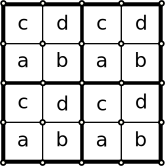
\includegraphics[scale=0.7]{quad_mesh_color_sym} \label{fig:quadCol}
	}
	\hspace{+1mm}
	\subfloat[]{
	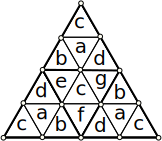
\includegraphics[scale=0.8]{triangle_mesh_color_sym} \label{fig:triaCol}
	}
	}
	\caption[Mesh element coloring]{Mesh element coloring showing two types of meshes. \protect\subref*{fig:quadCol} Structured quadrilateral mesh containing a total of four colors.  \protect\subref*{fig:triaCol}~Triangular mesh containing a total of six colors.}
	\label{fig:meshCol}
\end{figure}


\subsubsection{Partition-Parallel Message Scheduling}
Since \gls{acr:fem} elements exhibit geometrical locality in meshes, factor nodes adjacent to each other could be scheduled on the same processing element in order to compute using sequential updates; while communications between factor nodes in different processing elements can be scheduled using parallel updates.
This scheduling scheme is referred to as the \gls{acr:pps} and is illustrated in \figRef{fig:partPar}.
The nodes using the parallel schedule lie on the boundary of partitions.
As a result, the number of parallel scheduled nodes is considerably less than the number of sequentially scheduled nodes that lie in the interior of the partition.
A similar scheduling scheme was previously introduced in \chpRef{chp:PW-GaBP} and was referred to as the \gls{acr:hus} scheme \cite{bib:El-Kurdi2012EIOGBPSFLSDDLS}; however, the key distinction here is that the \gls{acr:cps} scheme can be used within each partition.

\begin{figure}
	\centering{
	\subfloat[]{
	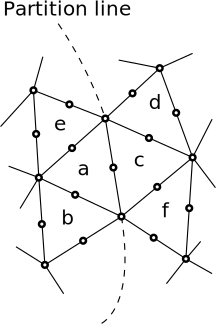
\includegraphics[scale=0.5]{partition_parallel_mesh} \label{fig:partParMesh}
	}
	\hspace{+2mm}
	\subfloat[]{
	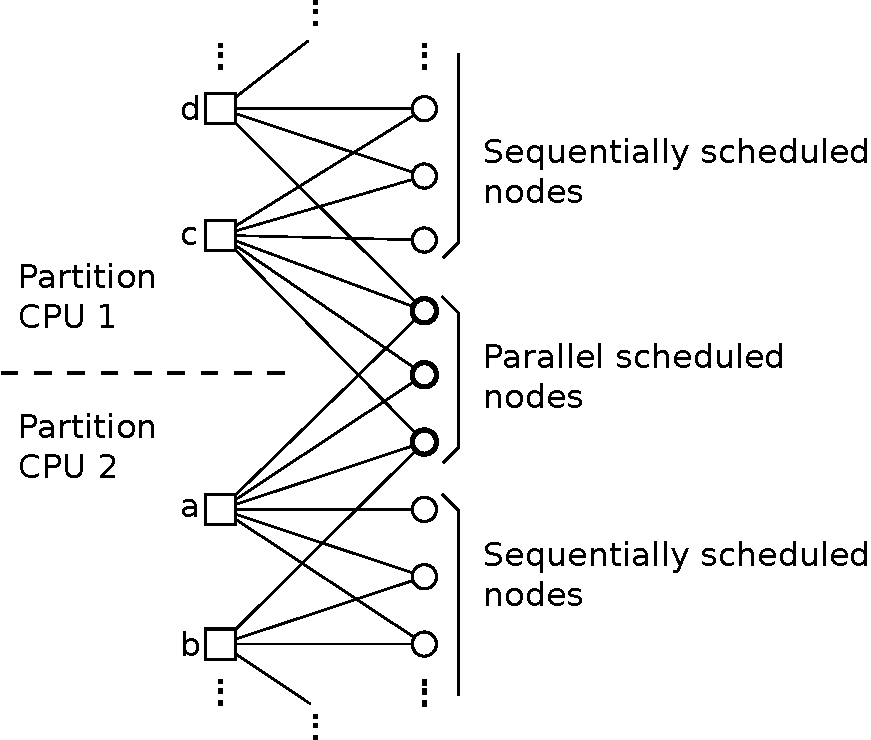
\includegraphics[scale=0.5]{partition_parallel_FG} \label{fig:partParFG}
	}
	}
	\caption[The partition-parallel Message schedule.]{The partition-parallel Message schedule. \protect\subref*{fig:partParMesh}~Hypothetical mesh. \protect\subref*{fig:partParFG}~Partitioned \gls{acr:femfg}. }
	\label{fig:partPar}
\end{figure}



\subsection{The FGaBP Algorithm Listing}
A high level listing of the \gls{acr:fgabp} algorithm is shown in \algRef{alg:FGaBP}.
The steps \ref{alg:genElmSrc} and \ref{alg:bndCnds} are considered the setup phase of the \gls{acr:fgabp} algorithm and can be performed completely in parallel.
The loop in line \ref{alg:partPar} reflects parallelism using partitions across CPUs in a cluster, which typically is programmed using \gls{acr:mpi}.
The loop in line \ref{alg:colPar} reflects parallelism using coloring across CPUs in a shared memory machine, which is programmed using multithreading.
\gls{acr:cps} implementations on shared memory machines can be performed by simply creating only one partition.
On the other hand, partition-parallel implementations can be performed by considering that each factor has its unique color; hence, the loop in line \ref{alg:colPar} is executed sequentially within a partition.
The \gls{acr:fgabp} algorithm, which encompasses a complete \gls{acr:fem} execution process, performs its computation completely in parallel without assembling or operating on any large sparse matrices.

\begin{algorithm}[h]
  %\centering
	\begin{algorithmic}[1]
		\STATE Obtain \gls{acr:fem} mesh
		\STATE Perform partition-color
		\STATE Generate element matrices $M_s$ and source vectors $B_s$ \label{alg:genElmSrc}
		\STATE Incorporate boundary conditions \label{alg:bndCnds}
		\STATE \textit{Initialize:} $\alpha_{ij} = 1,\,\, \beta_{ij} = 0,\,\,\forall i,j$
		\REPEAT[\gls{acr:fgabp} iteration: $t=1,2,\cdots$]
		\LOOP[Assign partitions to CPUs in cluster] \label{alg:partPar}
		\LOOP[For each color]
		\LOOP[Schedule factor nodes to all available CPU cores or threads] \label{alg:colPar}
		\STATE  Compute messages according to \eqnRef{eqn:vna}, \eqnRef{eqn:vnb}, \eqnRef{eqn:fnaO}, and \eqnRef{eqn:fnbO}
	\ENDLOOP
	\STATE Synchronize threads
\ENDLOOP
\STATE Synchronize parallel message buffers
\ENDLOOP
\UNTIL{Convergence check on messages}
\STATE \textit{Output:} $\mu_i = \frac{\beta_i}{\alpha_i}$
  \end{algorithmic}
  \caption{The \acrshort{acr:fgabp} algorithm.}
  \label{alg:FGaBP}
\end{algorithm}


%%%%%%%%%%%%%%%%%%%%%%%%%%%%%%%%%%%%%%%%%%%%%%%%%%%%%%%%%%%%%%%%%%%%%%%
%% Section
%%%%%%%%%%%%%%%%%%%%%%%%%%%%%%%%%%%%%%%%%%%%%%%%%%%%%%%%%%%%%%%%%%%%%%%


\section{Lower Complexity FGaBP}
\label{sec:lowerCompFGaBP}

As can be seen from the \gls{acr:fgabp} update rules in \eqnRef{eqn:vna}, \eqnRef{eqn:vnb}, \eqnRef{eqn:fnaO}, and \eqnRef{eqn:fnbO}, the \gls{acr:fgabp} computational complexity per iteration is dominated by the \gls{acr:fn} processes.
Because of the matrix inversion required by each \gls{acr:fn}, the total \gls{acr:fgabp} complexity per iteration, when using e.g. the Cholesky algorithm, is $\bigo{\gls{acr:nf} n (n-1)^3/3} \approx \bigo{\gls{acr:nf} n^4/3}$ where \gls{acr:nf} is the number of \glspl{acr:fn} in the \gls{acr:femfg} model.
For \gls{acr:fem} problems, \gls{acr:nf} is typically proportional to \gls{acr:nv}, where \gls{acr:nv} is the number of \glspl{acr:vn}.
In addition, we always have $n\ll \gls{acr:nf}$, e.g. for first order triangular meshes $n=3$ and first order tetrahedral meshes $n=4$.
More importantly, $n$ is independent of \gls{acr:nf} which implies that the \gls{acr:fgabp} algorithm can offer high parallel scalability for a good choice of message scheduling.
However, due to the high \gls{acr:fn} computational complexity, the local computational cost may dominate as $n$ increases when supporting higher degree FEM basis functions, for example when $n \geq 5$.
In the following, we present reformulations of the \gls{acr:fgabp} algorithm that considerably reduces the \gls{acr:fn} complexity to $\bigo{n^2}$.


We can reformulate the \gls{acr:fn} update rules using the partitioned matrix inversion identity as stated in the following:
\begin{equation}
	Z=\left[\begin{array}{cc}
		P & Q\\
		R & S
	\end{array}\right],\qquad Z^{-1}=\left[\begin{array}{cc}
		\tilde{P} & \tilde{Q}\\
		\tilde{R} & \tilde{S}
	\end{array}\right]
	\label{eqn:invPar}
\end{equation}
where:
\begin{align*}
	\tilde{P} & =V\\
	\tilde{Q} & =-VQS^{-1}\\
	\tilde{R} & =-S^{-1}RV\\
	\tilde{S} & =S^{-1}+S^{-1}RVQS^{-1}\\
	V & =\left(P-QS^{-1}R\right)^{-1}
\end{align*}
Comparing \eqnRef{eqn:invPar} to \eqnRef{eqn:wk} in the \gls{acr:fgabp} algorithm, we can see that $P = W^{(t_\star)}_{\mathcal{L}(i)}$, which is a single element matrix; and $R=Q^T=V$, which is a column matrix with dimensions $(n-1)\text{-by-}1$; and finally, $S = \bar{W}^{(t_\star)}$.
Then, the \gls{acr:fn} update rules can alternatively be obtained by directly computing the inverse of $W$ and partitioning it as follows:
\begin{align}
	(W^{(t_\star)})^{-1} & =\left[\begin{array}{cc}
		\tilde{W}_{\mathcal{L}(i)} & \tilde{C}^{T}\\
		\tilde{C} & \tilde{D}
	\end{array}\right] \label{eqn:fnInv}
\end{align}
The resulting \gls{acr:fn} updates will be:
\begin{align}
	\alpha_{ai}^{(t)} & =\frac{1}{\tilde{W}_{\mathcal{L}(i)}}-\alpha_{ia}^{(t_\star)} \label{eqn:fna2}\\
	\beta_{ai}^{(t)} & =B_{\mathcal{L}(i)}+\frac{1}{\tilde{W}_{\mathcal{L}(i)}}(\bar{K}^{(t_\star)})^{T}\tilde{C} \label{eqn:fnb2}
\end{align}
Using an in-place Cholesky inversion algorithm to compute $(W^{(t_\star)})^{-1}$, the \gls{acr:fn} complexity can be reduced to $\bigo{n^3/3}$.
Since $W$ is small and dense, optimized linear algebra libraries can be used to compute its inverse efficiently.
Examples of such libraries are Eigen~\cite{bib:eigen}, Gmm++~\cite{bib:gmm}, and Lapack~\cite{bib:lapack}.


For cases where $n$ is relatively large, e.g. $n\geq5$, computing the inverse can still be costly.
As shown by the \gls{acr:fem} distribution $\mathcal{P}$ in \eqnRef{eqn:statPoint}, the FEM solution requires only finding the marginal means as computed by the \gls{acr:fgabp} algorithm.
The marginal means are computed iteratively by the ratios of the nodal parameters $\beta_i$ and $\alpha_i$ as shown in \eqnRef{eqn:vnm}.
Substituting \eqnRef{eqn:vnb} into \eqnRef{eqn:fnb2} and rearranging terms we then obtain:
\begin{equation}
	\bar{u}_a^{(t)} = (W^{(t_\star)})^{-1} K^{(t_\star)} \label{eqn:locSol}
\end{equation}
which can be seen as the local element approximate solution obtained from the \fn{a} for the \vn{i} $i\in\mathcal{N}(a)$ and for fixed $\alpha$ messages.
If we partition $W$ as $W = D-E-F$ such that $D$ is the main diagonal of $W$, while $E$ and $F$ are the lower and the upper off-diagonals of $W$ correspondingly, a local stationary, fixed-point, iterative process can be created within each \gls{acr:fn}.
For example, the following will constitute a \gls{acr:gs} iteration:
\begin{equation}
	\bar{u}_a^{(t)} = (D-E)^{-1} F \bar{u}_a^{(t_\star)} + (D-E)^{-1} K^{(t_\star)}. \label{eqn:gsUpdate}
\end{equation}
Other fixed-point iterative methods such as Jacobi or \gls{acr:sor} can also be configured.


The $\alpha$ messages can be fixed after allowing the \gls{acr:fgabp} algorithm to execute normally for a couple of iterations, or until the $\alpha$ messages converge to a very high tolerance such as $10^{-1}$.
This should replace the initial values in the $\alpha$ messages with better estimates.
Then a number of iterations is executed using \eqnRef{eqn:locSol} to obtain a better estimate for $\bar{u}_a$.
In all of our experiments, one or two iterations of \gls{acr:gs} was practically sufficient.
Finally, the new $\beta_{ai}^{(t)}$ messages are obtained from the $\bar{u}_a^{(t)}$ estimates as follows:
\begin{equation}
	\beta_{ai}^{(t)} = \bar{u}_i^{(t)} \alpha_i^{(t_o)} - \beta_i^{(t_\star)} + \beta_{ai}^{(t_\star)}, \label{eqn:gsBetaUpdate}
\end{equation}
where $t_o$ is the iteration where the $\alpha$ messages are fixed.
Clearly, using this approach the \gls{acr:fn} process complexity is reduced to approximately $\bigo{n^2}$.
It can be shown that the fixed-point solutions, or marginal means, of the original \gls{acr:fgabp} update rules are equal to the fixed-point solutions of the new \gls{acr:fgabp} update rules.
However, the final message parameters, $\alpha$ and $\beta$, may be different between the two algorithms.
We refer to this reduced complexity algorithm as the \gls{acr:aufgabp} algorithm.
\tableRef{tbl:FGaBPUpdRules} summarizes the equations for the \gls{acr:fgabp} \gls{acr:fn} update rules and the associated computational complexity for a relatively large $n$.

\begin{table}
	\centering
	\begin{threeparttable}
		\caption{Summary of the \acrshort{acr:fgabp} update rules.} \label{tbl:FGaBPUpdRules}
		\begin{tabular}{lll} 
			\toprule
			Algorithm            & \gls{acr:fn} Update Equations                                                           & \gls{acr:fn} Complexity \tabularnewline
			\midrule
			Exact updates        & \eqnRef{eqn:fnaO}, \eqnRef{eqn:fnbO}                                                    & $O(n^4)$ \tabularnewline
			Exact updates        & \eqnRef{eqn:fna2}, \eqnRef{eqn:fnb2}                                                    & $O(n^3)$ \tabularnewline
			Approximated updates & \eqnRef{eqn:locSol}\tnote{1}, \eqnRef{eqn:gsUpdate}\tnote{2}, \eqnRef{eqn:gsBetaUpdate} & $O(n^2)$ \tabularnewline
			\bottomrule
		\end{tabular}
		\begin{tablenotes}
			\begin{footnotesize}
			\item[1] {Fixed $\alpha$ messages.}
			\item[2] {Using the \gls{acr:gs} iteration.}
			\end{footnotesize}
		\end{tablenotes}
	\end{threeparttable}
\end{table}


\section{Element Merging}
\label{sec:elmMerg}


In this section, variations on the graphical structure of the \gls{acr:fgabp} algorithm are proposed in order to increasing the parallel efficiency of the \gls{acr:fgabp} execution on multicore architectures with suitable cache capacities.
By virtue of the factorization structure of the \gls{acr:femfg} model, we can easily redefine new factors in \eqnRef{eqn:fgpf} by joining other factors as follows:
\begin{equation}
	\Psi_{\hat{s}}(U_{\hat{s}}) = \Psi_{s_1}(U_{s_1}) \Psi_{s_2}(U_{s_2}),
	\label{eqn:jpdf}
\end{equation}
where factors $s_1$ and $s_2$ are joint into factor $\hat{s}$, which is a function of the variable set $U_{\hat{s}} = U_{s_1} \cup U_{s_2}$.
Once suitable elements are identified for merging, the \gls{acr:fgabp} algorithm can be executed normally after locally assembling the merged elements' matrices and source vectors, $M_{\hat{s}}$ and $B_{\hat{s}}$ correspondingly.
When the factors are adjacent, the cardinality of $U_{\hat{s}}$ is $\cardinal{U_{\hat{s}}} = \cardinal{U_{s_1}} + \cardinal{U_{s_2}} - \cardinal{U_{s_1} \cap U_{s_2}}$.
If $U_{s_1}$ and $U_{s_2}$ are not adjacent, or disjoint, then $U_{s_1} \cap U_{s_2} = \emptyset$.
\Gls{acr:em} can be particularly advantageous if elements that share edges in 2D meshes or surfaces in 3D meshes are merged.
As a result, the memory bandwidth utilization can improve due to the considerable reduction in the total number of edges in the FEM-FG model. 
By merging adjacent elements, we can better utilize the high CPU computational throughput in exchange for the slower memory bandwidth and latency.


EM can be mainly useful for 2-D triangular and 3-D tetrahedral meshes with first order \gls{acr:fem} elements.
To quantify the effect of merging, we define the \gls{acr:mrr} percentage by dividing the amount of reduced memory from the merge by the original amount of memory before the merge.
The MRR is computed as:
\begin{equation}
	\OpN{MRR} = \frac{\sum_{a \in \mathcal{D}}M_a - \sum_{a \in \mathcal{C}}M_a}{\sum_{a \in \mathcal{D}}M_a} \cdot 100\%,
\end{equation}
where $\mathcal{D}$ is the set of all factors before any merge, $\mathcal{C}$ is the set of merged factors, and $M_a$ is the amount of memory required for \fn{a}.
As later shown in \secRef{sec:fgabpImp}, the memory complexity per \gls{acr:fn} can be obtained by $M_i \propto \bigo{4n_a+n_a^2}$ where $n_a$ is the number of \fn{a} edges, or the rank of $M_a$.
If we consider structured meshes for illustration purposes only, the resulting \gls{acr:mrr} is 23.8\% when merging every two adjacent triangles into a quadrilateral, or 46.4\% when merging every four fully connected triangles into a quadrilateral.
\figRef{fig:elm_merge} illustrates the different \gls{acr:femfg} graphs resulting from merging every two or every four adjacent triangles in a structured triangular mesh.


For irregular triangular meshes with large numbers of triangles, the Euler's formula \cite[p.~28]{bib:Berg2008CGA} states that each vertex will be surrounded by six triangles on average.
Thus, when merging mostly six triangle groups into hexagons, the \gls{acr:mrr} increases, on a per merge basis, to 38.9\%, or to 42.9\% when merging five triangles.
Merging triangles does not have to be uniform.
We may decide to merge patches of 2, 3, 4, 5, 6, or more as long as the triangles share edges and form connected or, preferably, convex regions.
Similarly for 3D tetrahedral meshes, merging tetrahedrons sharing faces can also result in significant memory storage reductions.
If two tetrahedrons of first order are merged, the \gls{acr:mrr} is 29.7\%, and 53.1\% when merging three tetrahedrons sharing faces and are enclosed by five vertices.


\def \MyVariableScale{.7}
\def \MyVariableSeparation{1cm}
\begin{figure}[h]
	\centering
	{
	\subfloat[]{%
	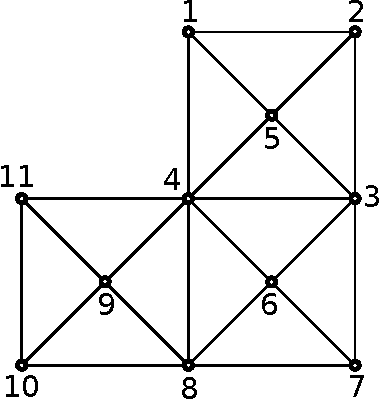
\includegraphics[scale=\MyVariableScale]{fg_triangle_merge_a} \label{fig:elm_merge_a}
	}
  %\hfil
	\hspace{\MyVariableSeparation}
	\subfloat[]{%
	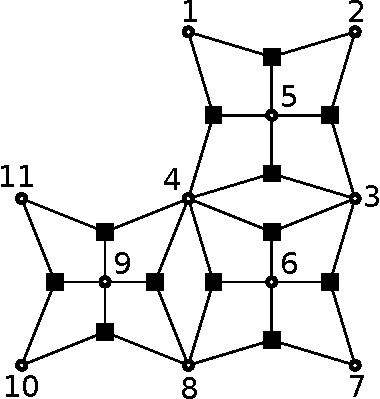
\includegraphics[scale=\MyVariableScale]{fg_triangle_merge_b} \label{fig:elm_merge_b}
	}
	\vfill
	\subfloat[]{%
	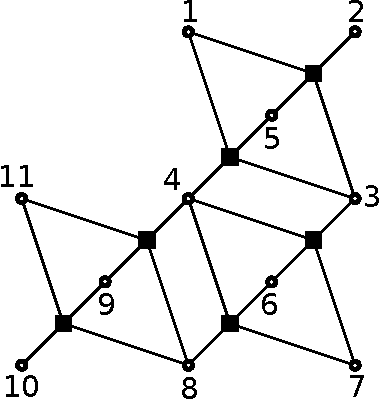
\includegraphics[scale=\MyVariableScale]{fg_triangle_merge_c} \label{fig:elm_merge_c}
	}
  %\hfil
	\hspace{\MyVariableSeparation}
	\subfloat[]{%
	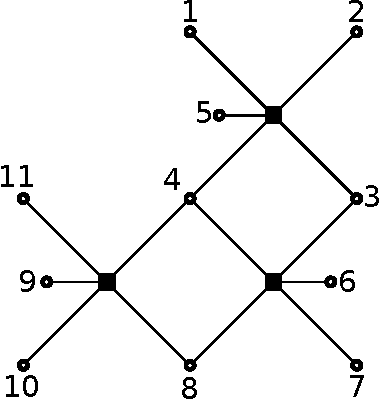
\includegraphics[scale=\MyVariableScale]{fg_triangle_merge_d} \label{fig:elm_merge_d}
	}
	}
	\caption[Element merging examples.]{Triangular element merging examples. \protect\subref*{fig:elm_merge_a}~Original triangular mesh. \protect\subref*{fig:elm_merge_b}~The initial \gls{acr:femfg} using single element factorization. \protect\subref*{fig:elm_merge_c}~Merging two adjacent triangles. \protect\subref*{fig:elm_merge_d}~Merging adjacent four triangles.}
	\label{fig:elm_merge}
\end{figure}


While merging elements based on a structured mesh is a trivial operation, we can still efficiently merge certain element configurations in unstructured meshes with the aid of partitioning algorithms \cite{bib:parmetis2013,bib:parmetisMan,bib:metis,bib:parmetisKarypis1996}.
For such cases, the partitioning algorithms can be used to isolate the desired patches of elements.
Specifically, the work in \cite{bib:ChanAgg} presents algorithms to create macro-elements by joining adjacent elements in unstructured grids.
Partitioning may add some overhead in the preprocessing stage; however, since in practice the number of factors is much greater than the number of CPU cores, a lower partition quality can be used to lower the partitioning overhead time \cite{bib:parmetisMan} without having much impact on the overall parallel efficiency.

The element merging does not affect the underlying FEM mesh discretization properties, it does however affect the \gls{acr:fgabp} numerical complexity as a solver.
Our results in \secRef{sec:elmMergRes} reveal that the overall computational complexity of the merged \gls{acr:femfg} can be higher than that of the original, un-merged one.
Nonetheless, the \gls{acr:fgabp} demonstrates considerable speedups for the merged \gls{acr:femfg} structure, because of better utilization of available memory bandwidth and cache resources resulting from an improved computational locality.
These observations are illustrated in \secRef{sec:elmMergRes}.
To conclude, we propose to use the merge feature as a high-level means to control trade-offs between CPU resources such as memory bandwidth, cache utilization, and CPU cycles to facilitate fine-tuned implementations on manycore architecture.


\section{Implementation}
\label{sec:fgabpImp}

\subsection{Data-structures}
\label{sec:fgabpDS}

Using the \gls{acr:cps} scheme of \gls{acr:fgabp} and assuming all \glspl{acr:fn} are of the same size, the overall storage requirement of \gls{acr:fgabp} is $\bigo{2 \gls{acr:nv}+\gls{acr:nf}(n^2+4n)}$ in 64-bit words.
This includes two vectors of size \gls{acr:nv} for the \gls{acr:vn}'s $\alpha_i$ and $\beta_i$, and a data-structure of size \gls{acr:nf} containing the \glspl{acr:fn} data-structures where each \gls{acr:fn}'s data-structure contains a dense matrix $M_a$, vectors $B_a$, $\alpha_{ai}$, and $\beta_{ai}$, and a 64-bit integer vector storing local to global index associations.
This setup, also, assumes that all indices are stored in 64-bit integers and all real numbers are stored in 64-bit \gls{acr:dpfp}, which is essential for very large problems.
Since usually $\bigo{\gls{acr:nf}}\approx \bigo{\gls{acr:nv}}$, the overall \gls{acr:fgabp} memory complexity is $\bigo{\gls{acr:nv}}$, typical for sparse problems.
However, unlike conventional sparse data-structures such as the \gls{acr:csr}, all the \gls{acr:fgabp} data is contiguous, or dense.
Hence, the \gls{acr:fgabp} data-structure adds minimal overhead by eliminating the need to store complicated sparsity patterns.
For certain cases where the problem size does not require 64-bit indices, e.g. when approximately $10^6<\gls{acr:nv}<10^8$, 32-bit indices can be used instead.
For such a case, the \gls{acr:fgabp} memory complexity will be slightly lower to $\bigo{2 \gls{acr:nv}+\gls{acr:nf}(n^3+2.5n)}$.


In order to compare the \gls{acr:fgabp} data-structure with the other sparse data-structures in terms of storage size, we use the \gls{acr:srm} as follows:
\begin{align}
	\OpN{\acrshort{acr:srm}} & = \frac{\text{Other sparse storage}}{\text{\gls{acr:fgabp} storage}}\\
	& = \frac{2 \gls{acr:nnz} +2 \gls{acr:nv}}{2 \gls{acr:nv}+\gls{acr:nf}(n^3+4n)}. \label{eqn:srmCSR}
\end{align}
In \eqnRef{eqn:srmCSR} we are considering the \gls{acr:csr} storage size as an example for comparison due to its popularity.
As shown in \figRef{fig:csr}, the size of the \gls{acr:csr} format includes a vector of size \gls{acr:nv} for the row start index, and two vectors of size \gls{acr:nnz} for the element value and its row index. 
In addition, the right-hand-side vector of size \gls{acr:nv} is added to the \gls{acr:csr} format, in order to provide a consistent comparison with the \gls{acr:fgabp} format which already includes the elements' source vectors in its storage.
It is important to note that in practice the sparse storage for other solvers is typically much larger than what is used here in the \gls{acr:srm}; since, iterative solvers such as the \gls{acr:pcg}, as in \algRef{alg:pcg}, would required additional memory to store the preconditioner as well as the search and residual vectors.
On the other hand, the \gls{acr:fgabp} data-structure includes all the information needed to solve the \gls{acr:fem} problem rather than just storing the sparse matrix of the global linear system.
However, since implementations of the \gls{acr:pcg} algorithm may vary from one library to another, we will not consider its full storage in the \gls{acr:srm} analysis, but rather only the storage required for the sparse matrix and the right-hand-side vector.

\subsection{The FEM-FG Edges}

Another metric we use in our analysis is the \gls{acr:lrm} defined as follows:
\begin{align}
	\OpN{\acrshort{acr:lrm}} & = \frac{\text{Number of edges in the \gls{acr:pwgm}}}{\text{Number of edges in the \gls{acr:femfg} model}}\\
	& = \frac{(\gls{acr:nnz}-\gls{acr:nv})/2}{\gls{acr:nf} n}.
\end{align}
The \gls{acr:lrm} is a measure for the amount of information the algorithm is required to communicate per iteration.
As we will see later in \secRef{sec:fgabpRes}, this ratio may explain some of the convergence behavior of \gls{acr:fgabp} in comparison to other sparse algorithms.
It is important to note that the \gls{acr:lrm} is not a measure for the memory bandwidth requirement of a particular algorithm.
The \gls{acr:srm} may be a closer measure to the memory bandwidth required by the solver per iteration.
However, the memory bandwidth is not easy to measure because, not only does it depends on the amount of data needed to be accessed, but rather it depends more on the access pattern of the sparse data-structure.
That is because at the hardware level, the memory controllers respond to the CPU's memory requests by sending data in contiguous chunks, as in memory lines, which is stored temporarily in the cache memory \cite{bib:Hennessy2012CAQA}. 
The CPU on the other hand, uses the cache memory to retrieve exactly what it needs.
This is the key reason behind the notoriously poor performance of sparse data-structures.
If the data is not contiguous in memory, then the CPU only utilizes a small fraction of the data transfer to the cache.
This leads to under-utilized cache or poorly utilized memory bandwidth causing an overall poor computational throughput.
The \gls{acr:fgabp}, on the other hand, utilizes contiguous data-structures which considerably improves its memory bandwidth utilization.

\tableRef{tbl:FEMFGAnal} illustrates the \gls{acr:srm} and the \gls{acr:lrm} trends for a number of meshes.
The L-shaped domain is used as the example domain.
The open-source software \libName{Gmsh} \cite{bib:gmsh2009} is used to mesh the domain.
The triangular, tetrahedral and quadrilateral meshes are unstructured, while the hexahedral meshes are structured and also generated by \libName{Gmsh}.
The stiffness matrix was obtained for the Laplace equation using the software package \libName{GetFEM} \cite{bib:getfem}.
Using the stiffness matrix, we can obtain the number of edges for the corresponding \gls{acr:pwgm} using the actual \gls{acr:nnz} of the matrix.
Clearly, for both ratio metrics the \gls{acr:fgabp} shows a progressively increasing advantage as the \gls{acr:fem} order increases for all types of meshes.
In particular, the \gls{acr:lrm} shows considerable advantage for all types of meshes except the first order triangular and tetrahedral meshes.
However, this can be efficiently remedied using the \gls{acr:em} feature discussed earlier in \secRef{sec:elmMerg}.

%%%%%%%%%%%%%%%%%%%
%% This table is rotated in landscape mode
%%%%%%%%%%%%%%%%%%
\afterpage{%
\clearpage% Flush earlier floats (otherwise order might not be correct)
%\thispagestyle{empty}% empty page style (?)
\begin{sidewaystable}% Landscape page
	%\begin{table}[t]
	\centering
	\begin{threeparttable}[t]
		\caption{The \acrshort{acr:femfg} comparison analysis.} \label{tbl:FEMFGAnal}
		\begin{tabular}{lrrrrrrrr>{\itshape}r>{\itshape}r} 
			\toprule
			\multicolumn{1}{c}{Element}& \multicolumn{1}{c}{$n$ \tnote{1}}& \multicolumn{1}{c}{\gls{acr:nv}}& \multicolumn{1}{c}{\gls{acr:nf}}& \multicolumn{1}{c}{\gls{acr:nnz}}& \multicolumn{1}{c}{\acrshort{acr:pwgm}}& \multicolumn{1}{c}{Sparse}& \multicolumn{1}{c}{\acrshort{acr:femfg}}& \multicolumn{1}{c}{\acrshort{acr:femfg}}& \multicolumn{1}{c}{\acrshort{acr:srm}}& \multicolumn{1}{c}{\acrshort{acr:lrm}} \tabularnewline
			\multicolumn{1}{c}{Geometry}& & &  &  & \multicolumn{1}{c}{Edges}& \multicolumn{1}{c}{Storage\tnote{2}}& \multicolumn{1}{c}{Edges}& \multicolumn{1}{c}{Storage \tnote{3}}&  & \tabularnewline
			\midrule
			triangle      & 3  & 349   & 634  & 2313    & 982     & 6372    & 1902   & 14012   & 0.45 & 0.52 \tabularnewline
			triangle      & 6  & 1331  & 634  & 14831   & 6750    & 36318   & 3804   & 40702   & 0.89 & 1.77 \tabularnewline
			triangle      & 10 & 2947  & 634  & 48967   & 23010   & 112670  & 6340   & 94654   & 1.19 & 3.63 \tabularnewline
			triangle      & 15 & 5197  & 634  & 119937  & 57370   & 265860  & 9510   & 191084  & 1.39 & 6.03 \tabularnewline
			triangle      & 3  & 1092  & 2070 & 7414    & 3161    & 20289   & 6210   & 45654   & 0.44 & 0.51 \tabularnewline
			triangle      & 6  & 4253  & 2070 & 48059   & 21903   & 117384  & 12420  & 132706  & 0.88 & 1.76 \tabularnewline
			triangle      & 10 & 9484  & 2070 & 159196  & 74856   & 365813  & 20700  & 308768  & 1.18 & 3.62 \tabularnewline
			triangle      & 15 & 16785 & 2070 & 390505  & 186860  & 864936  & 31050  & 623520  & 1.39 & 6.02 \tabularnewline
			quadrilateral & 4  & 1057  & 1000 & 9169    & 4056    & 23624   & 4000   & 34114   & 0.69 & 1.01 \tabularnewline
			quadrilateral & 9  & 4113  & 1000 & 64449   & 30168   & 149464  & 9000   & 125226  & 1.19 & 3.35 \tabularnewline
			quadrilateral & 16 & 9169  & 1000 & 225841  & 108336  & 497528  & 16000  & 338338  & 1.47 & 6.77 \tabularnewline
			tetrahedron   & 4  & 689   & 2668 & 8343    & 3827    & 20132   & 10672  & 86754   & 0.23 & 0.36 \tabularnewline
			tetrahedron   & 10 & 4521  & 2668 & 112989  & 54234   & 248584  & 26680  & 382562  & 0.65 & 2.03 \tabularnewline
			tetrahedron   & 20 & 14165 & 2668 & 619257  & 302546  & 1309340 & 53360  & 1308970 & 1.00 & 5.67 \tabularnewline
			hexahedron    & 8  & 2448  & 1815 & 54400   & 25976   & 121041  & 14520  & 179136  & 0.68 & 1.79 \tabularnewline
			hexahedron    & 27 & 16951 & 1815 & 966985  & 475017  & 2018726 & 49005  & 1553057 & 1.30 & 9.69 \tabularnewline
			hexahedron    & 8  & 4896  & 3993 & 115574  & 55339   & 255629  & 31944  & 393120  & 0.65 & 1.73 \tabularnewline
			hexahedron    & 27 & 35443 & 3993 & 2099065 & 1031811 & 4375346 & 107811 & 3413027 & 1.28 & 9.57 \tabularnewline
			\bottomrule
		\end{tabular}
		\begin{tablenotes}
			\begin{footnotesize}
			\item[1] {$n$ is the number of variables per element.}
			\item[2] {Using \gls{acr:csr} format.}
			\item[3] {All storage estimates are in the order of \gls{acr:dpfp} numbers.}
			\end{footnotesize}
		\end{tablenotes}
	\end{threeparttable}
	%\end{table}
\end{sidewaystable}
\clearpage% Flush page
}

For certain cases, the \gls{acr:lrm} data can be analytically explained.
Considering the Euler theorem \cite[p.~28]{bib:Berg2008CGA} for triangular meshes of the first order, the ratio of edges to elements is $3/2$, now dividing by the number of factor variables (which is $n=3$ for triangular factors), then the resulting ratio should be $0.5$ as predicted by the tabulated results for first order triangles.
If we consider approximating the unstructured quadrilateral mesh with a regular one, with uniform gird points, and noting that for an isolated quadrilateral element there are six \gls{acr:fem} edge couplings, then the ratio of edges to elements approaches 4 which explains the 1.01 ratio.
Similarly for hexahedral meshes on cubical domains of dimension $N$, the number of edges for $N^3$ hexahedrons approaches $14N^3 + \bigo{N^2}$ leading to a ratio of $14/8$ which explains the 1.79 and 1.73 ratios.


\subsection{CPU Multicore Implementation}

The \gls{acr:fgabp} code was designed using C++ \gls{acr:oop} \cite{bib:c++stroustrup2013,bib:c++prata2004}.
The \gls{acr:oop} based design of the \gls{acr:fgabp} software facilitates its integration with existing frameworks of open-source libraries such as \dealName{} \cite{bib:dealii2007} and \libName{GetFEM++} \cite{bib:getfem}.
The following section presents the numerical results on the performance of both the basic \gls{acr:fgabp} and the modified \gls{acr:aufgabp} algorithms.
We utilize meshes and \gls{acr:fem} setup generated from three open-source libraries, which are \libName{Gmsh}, \libName{GetFEM++}, and \dealName{}.
We validate the \gls{acr:fgabp} algorithms on both regular and irregular meshes using various \gls{acr:fem} interpolation orders and geometrical elements shapes such as triangles, quadrilaterals, and hexahedrons.
We utilize 2D and 3D domains with various boundary conditions.


For CPU multicore implementations, the \libName{OpenMP} \cite{bib:openmp} standard \gls{acr:api} is used to parallelize the \gls{acr:fgabp} code.
Using the \gls{acr:cps} scheme, the color loops are parallelized such that each thread executes a \gls{acr:fn} routine.
Thread synchronization directives are used only at the execution end of each color group; that is, the number of synchronization directives is equal to the number of color groups in the \gls{acr:cps} scheme.


\section{The FGaBP Numerical Results and Discussions}
\label{sec:fgabpRes}

\subsection{FGaBP Verification}
\label{sec:fgabpVer}

In this section, we verify the numerical results of the new \gls{acr:aufgabp} formulation using the definite Helmoltz problem with known solution as provided by the \dealName{} library for 2D and 3D domains as well as higher order \gls{acr:fem} elements.
The definite Helmholtz is formulated as follows:
\begin{align}
	-\nabla\cdot\nabla u+ u &= g, \text{ on } \Omega \label{eqn:Helm}\\
	u &= f_1, \text{ on } \partial D \label{eqn:HelmD}\\
	\textbf{n}\cdot \nabla u &= f_2, \text{ on } \partial N \label{eqn:HelmN}
\end{align}
where $\partial D$ and $\partial N$ are the Dirichlet and Neumann boundaries such that $\partial D \cup \partial N = \partial \Omega$, and $\Omega$ is the square or cubic domain bounded by $[-1,1]$.
Equation \eqnRef{eqn:HelmN} constitutes the non-homogeneous Neumann boundary condition.
The right-hand-side functions are set, such that the exact solution is:
\begin{equation}
	u(p) = \sum_i^3 \exp\left( - \frac{| p - p_i |^2}{\sigma^2} \right)
	\label{eqn:exactSol}
\end{equation}
where $p$ is a spatial variable in $(x,y,z)$, $p_i$ are exponential center points chosen arbitrarily, and $\sigma = 0.125$.
The library \dealName{} creates the mesh, and provides the \gls{acr:fgabp} class with the elements' $M_s$, $B_s$ matrices, as well as, the local to global index data.
The \gls{acr:fgabp} processes the \gls{acr:fem} problem element-by-element in parallel and sends the end solution back to \dealName{} which computes the final error relative to the exact solution.



The \gls{acr:aufgabp} uses $\alpha$ message tolerance of $10^{-1}$ and two GS iterations.
The test cases are obtained by varying the \gls{acr:fem} element order from the 1\ssst to the 3\ssrd order for both 2D quadrilaterals and 3D hexahedrals.
\figRef{fig:HelmRes} shows the error plots for each test case.
The global error for each test case is obtained by summing the squares of the $l^2$-norm error of each element and then taking the square root of that value.
It can be seen that the \gls{acr:aufgabp} obtains the expected error trends for the \gls{acr:fem} showing increased accuracy on all test cases for both trends of increasing number of elements as well as increasing \gls{acr:fem} order.

\begin{figure}[t]
	\centering{
	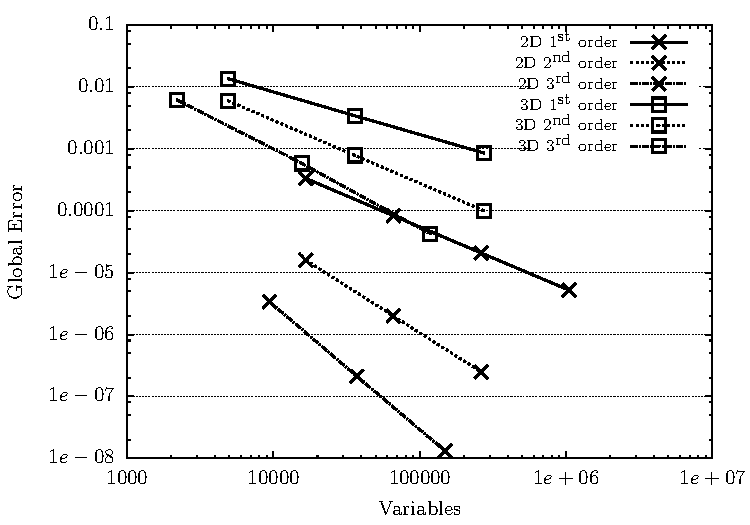
\includegraphics[scale=1.3]{plot_Helm_2D3D.pdf}
	}
	\caption[The global error performance of the AU-FGaBP.]{The global error of the AU-FGaBP obtained from element-based $l^2$-norm error relative to the exact solution.}
	\label{fig:HelmRes}
\end{figure}


\subsection{Performance Comparison}

The \gls{acr:fgabp} algorithm performance is demonstrated by solving Poisson's equation on a \gls{acr:ssc} with two dielectric media as shown in \figRef{fig:msf}.
The domain includes Dirichlet and homogeneous Neumann boundary conditions and is meshed with an irregular triangular mesh.
Different trials are performed by increasing the order of the \gls{acr:fem} interpolation from the 1\ssst order to the 5\ssth order while reducing the number of elements so as to keep the number of unknowns approximately similar.
As can be seen from the \gls{acr:lrm} data, the \gls{acr:femfg} model reduces memory communication for element orders greater than one by reducing the number of nodal links in the resulting \gls{acr:femfg} model compared to solvers such as the \gls{acr:pwgabp}.
With respect to algebraic solvers such as the \gls{acr:cg}, the link number directly correlates with the required memory communication.

\begin{figure}[t]
	\centering
	{
  %\hspace{-1mm}
	\subfloat[]{%
	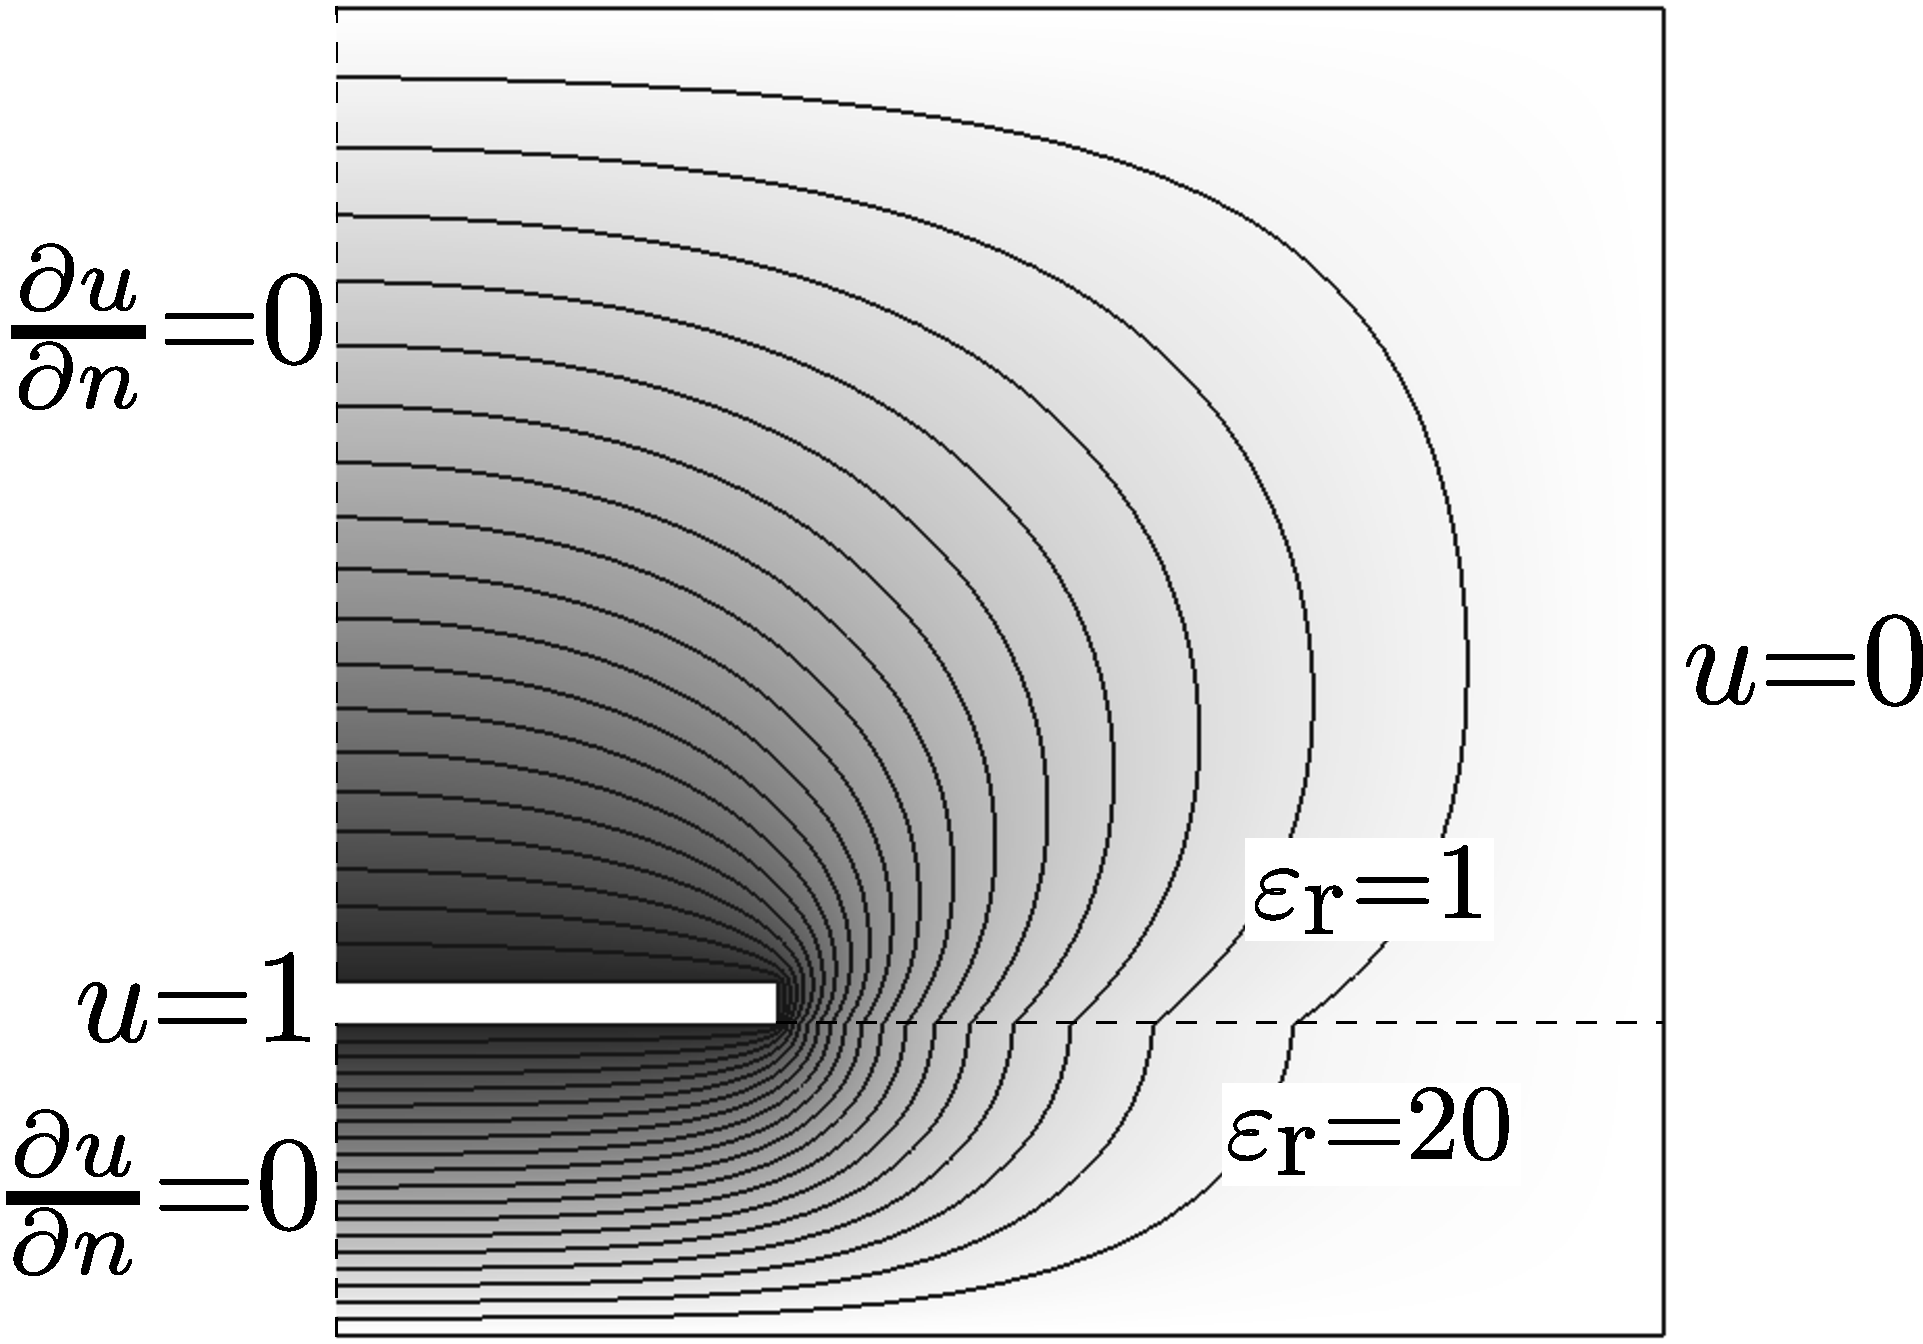
\includegraphics[scale=0.2]{FIG8}
	\label{fig:msf}
	}
	\hspace{+4mm}
	\subfloat[]{%
	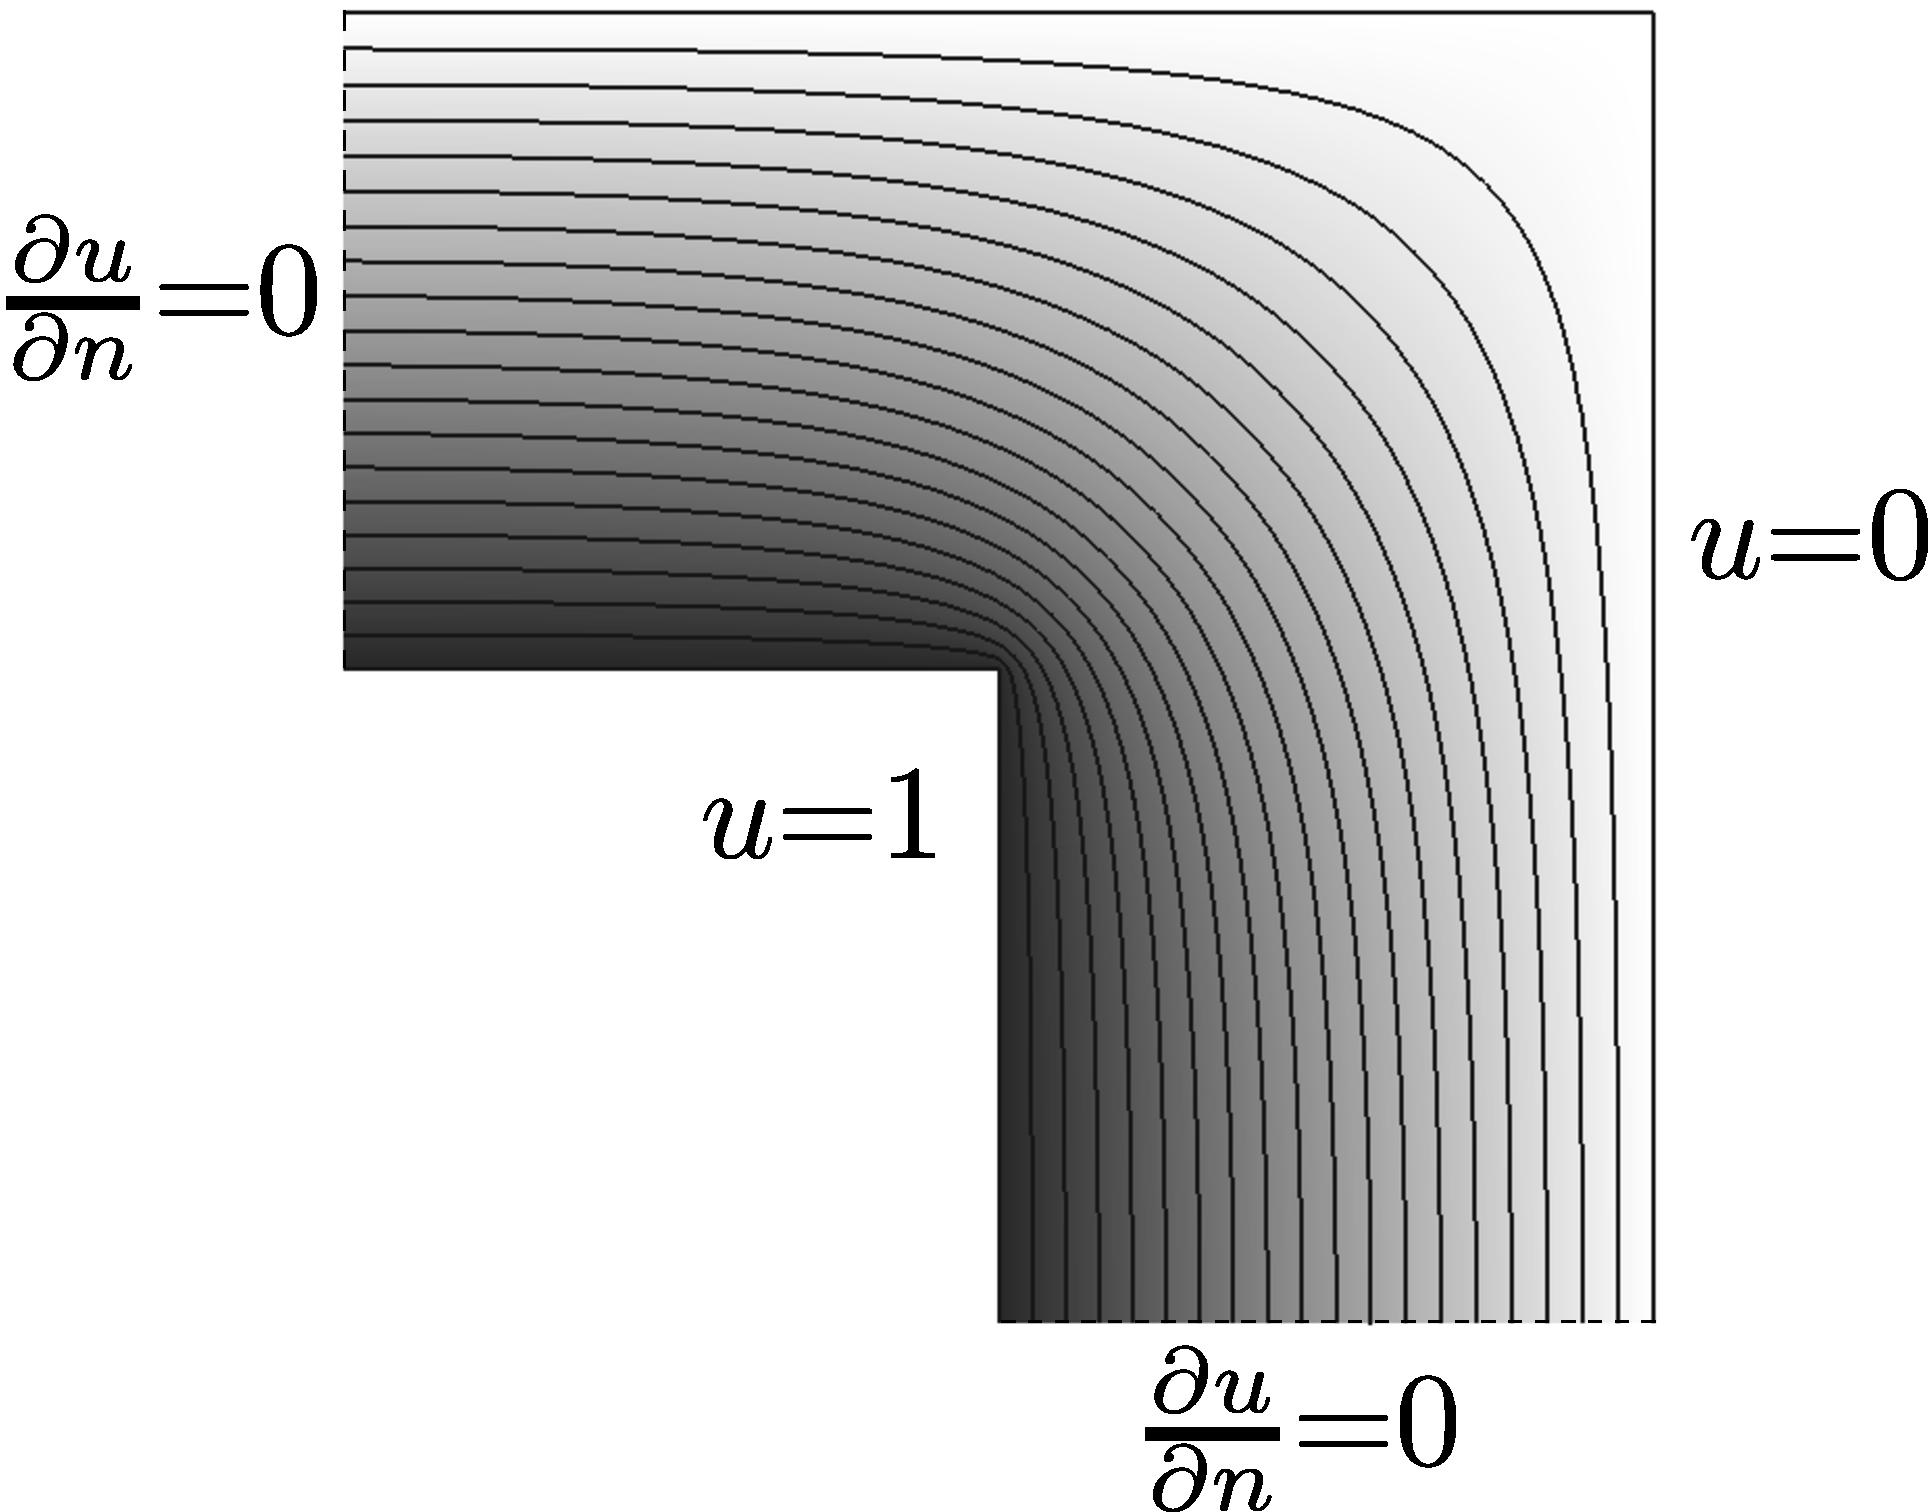
\includegraphics[scale=0.18]{FIG9}
	\label{fig:lsf}
	}
	}
	\caption[The Laplace equipotential contour lines.]{The Laplace equipotential contours obtained using \gls{acr:fgabp}, the dimensions of both structures are within the unit interval $\left[ 0,1 \right]$ cm. \protect\subref*{fig:msf} The right symmetrical side of the shielded strip between two different materials. \protect\subref*{fig:lsf} The top-right symmetrical corner of the square coaxial conductor.}
	\label{fig:ps}
\end{figure}


Also shown in \tableRef{tbl:FGaBPRes} are the iteration results of the \gls{acr:fgabp}, the \gls{acr:pwgabp}, and the \gls{acr:dpcg}.
The iterations were terminated on all experiments when the $l^2$-norm was dropped to $10^{-9}$.
We used our automatic relaxation scheme, previously introduced in \chpRef{chp:relGaBP}, to accelerate the convergence of both the \gls{acr:pwgabp} and the \gls{acr:fgabp}.
The \gls{acr:pwgabp} used \gls{acr:nmr}; whereas, the \gls{acr:fgabp} used \gls{acr:emr}.
It is important to note that the \gls{acr:pwgabp} and the \gls{acr:dpcg} require global large sparse matrix operations in each iteration which limit their effectiveness for parallel implementations; while in contrast, the \gls{acr:fgabp} requires completely decoupled computations performed element-by-element.
The last column of \tableRef{tbl:FGaBPRes} shows the \gls{acr:su} results of \gls{acr:fgabp} using a \gls{acr:cps} implementation on a quad-core CPU over the sequential one on the same workstation.
Although the implementation was not optimized to take advantage of specialized CPU features, the \gls{acr:fgabp} illustrated increased efficiency of parallel implementation as the interpolation order increases.
This is due to the \gls{acr:fgabp} making good use of increased localized computations and reduced memory communications which is a direct result from the \gls{acr:femfg} graph that reduces nodal links.


While the \gls{acr:dpcg} algorithm demonstrated the lowest iteration count, the \gls{acr:fgabp} algorithm demonstrated a trend of reducing number of iterations as the \gls{acr:fem} order increases; which illustrates its increased computational stability.
This is mainly due to the \gls{acr:fgabp} algorithm performing localized computations on small dense matrices up to order 5 instead of operating on very large sparse matrices that become increasingly ill-conditioned as the order of the \gls{acr:fem} interpolation increases.
This is a key advantage in comparison to algebraic based solvers such as the \gls{acr:pcg} whose iteration count increases as the condition number of the global characteristic matrix increases due to increasing \gls{acr:fem} order.


Even though at this stage, the \gls{acr:fgabp} algorithm does not seem to be competitive enough with the \gls{acr:pcg} solver iteration-wise, this problem will be remedied by introducing a multigrid scheme for the \gls{acr:fgabp} algorithm as will be shown later in \chpRef{chp:FMGaBP}. 
Lastly, as can also be seen in \tableRef{tbl:FGaBPRes}, the \gls{acr:pwgabp} failed to converge as the interpolation order increased beyond the 2\ssnd order, since the resulting global matrix is becoming increasingly ill-conditioned.
In contrast, the \gls{acr:fgabp} successfully converged for all cases demonstrating a significant improvement over the \gls{acr:pwgabp}, and likewise the \gls{acr:gs} and the \gls{acr:sor} solvers.
This result may be attributable to the structure induced by the \gls{acr:femfg} model, which, unlike the \gls{acr:pwgm} model, factors the graph over cliques causing the \gls{acr:fn} computation in the \gls{acr:fgabp} to correlate more local variables which increases the stability of the overall algorithm.
Fundamentally, factoring the graph over cliques significantly reduces the number of loops in the graph which causes the \gls{acr:bp} computation to be more stable.
This result incites further investigation on the convergence behavior of Gaussian \gls{acr:bp} type algorithms for both the \gls{acr:femfg} model as well as general \glspl{acr:gm}.


\begin{table}[h]
	\centering
	\caption{Shielded microstrip results for \acrshort{acr:fgabp}, \acrshort{acr:pwgabp}, and \acrshort{acr:dpcg}.} \label{tbl:FGaBPRes}
	\begin{threeparttable}[c]
		\begin{tabular}{l r r r r r r>{\itshape} r}
			\toprule
			Order & \gls{acr:nv} & \gls{acr:nf} & \gls{acr:lrm} & \gls{acr:pwgabp} & \gls{acr:dpcg} & \gls{acr:fgabp} & CPU \tabularnewline
			&              &              &               & itrs \tnote{1}   & itrs           & itrs            & SU \tnote{2} \tabularnewline
			\midrule
			1\ssst & 10076 & 19252 & 0.46 & 542  & 239 & 1486 & 1.1 \tabularnewline
			2\ssnd & 9818  & 4787  & 1.67 & 3582 & 379 & 3221 & 1.3 \tabularnewline
			3\ssrd & 10108 & 2191  & 3.42 & -    & 447 & 1762 & 2.1 \tabularnewline
			4\ssth & 10131 & 1237  & 5.69 & -    & 608 & 1564 & 3.2 \tabularnewline
			5\ssth & 10056 & 786   & 8.44 & -    & 826 & 1362 & 3.4 \tabularnewline
			\bottomrule
		\end{tabular}
		\begin{tablenotes}
			\begin{footnotesize}
			\item[1] {\footnotesize The shorthand itrs refers to iterations.}
			\item[2] {\footnotesize The speedup is relative to sequential \gls{acr:fgabp}.}
			\end{footnotesize}
		\end{tablenotes}
	\end{threeparttable}
\end{table}


\subsection{FGaBP Convergence Trends}
\figRef{fig:fgabpItr} shows the convergence behavior of the \gls{acr:fgabp} for 2D and 3D meshes of quadrilateral and hexahedral elements.
The \gls{acr:fem} problem is solving Laplace on the L-shaped domain \figRef{fig:lsf}.
The \gls{acr:fem} assembly function was performed using the open-source library \dealName{} \cite{bib:dealii2007}.
Clearly, the \gls{acr:fgabp} displays near linear convergence with increasing problem size.
Note that, the slight variations in the trends are mainly due to the automatic relaxation algorithm.
In addition, the \gls{acr:fgabp} showed similar trends of lower number of iterations as the complexity of the local factors increased either in terms of space dimension or \gls{acr:fem} order.

\begin{figure}
	\centering
	{%
	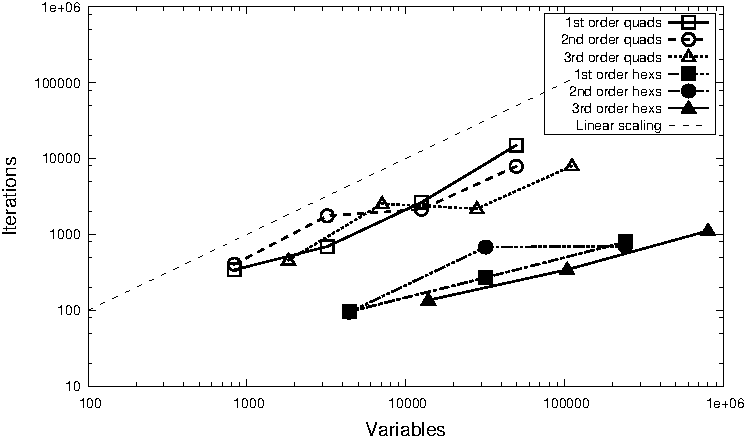
\includegraphics[scale=1.2]{FGaBP_itrs}
	}
	\caption{The \acrshort{acr:fgabp} algorithm executed on quadrilateral and hexahedral meshes of different orders.}
	\label{fig:fgabpItr}
\end{figure}


\subsection{Element Merging Performance}
\label{sec:elmMergRes}

The \gls{acr:em} feature implemented with the \gls{acr:fgabp} algorithm is demonstrated using a structured triangular mesh on a unit square domain.
The Laplace equation is solved in the domain using zero Dirichlet on the boundary.
The unit square is subdivided into equally spaced sub-squares where each square is further divided into two right triangles.
We perform two levels of merges by merging each two adjacent triangles, and then each four adjacent triangles.
The original mesh has $N_f=200000$ triangular element \glspl{acr:fn}.
Relaxation was not used in order to isolate the effect of merging on the iteration count.
The algorithm iterations were terminated when the message relative $l^2$-norm reached $<10^{-9}$.
\tableRef{tbl:fgabpMerge} shows the speedup results of the merges.
Execution was performed on an Intel Core2 Quad CPU with clock frequency of 2.83 GHz.


The merge results in increasing speedups.
Noting the overall computational complexity of the measured algorithm is approximately $\bigo{TN_f(n^3 + n^2)}$, where $T$ is the total number of iterations, the overall computational complexity of the merged algorithms has actually increased as can be noted by the complexity ratio column.
However, the execution time was actually faster which was mainly due to the improved locality of the algorithm. 
This improved locality results in better trade-offs of cache and memory bandwidth for cheaper CPU flops.

\begin{table}
	\centering
	\begin{threeparttable}
		\caption{AU-FGaBP with Element Merge Speedups.} \label{tbl:fgabpMerge}
		\begin{tabular}{lrrrr>{\itshape}r} \toprule
			Merge       & $N_f$  & $n$ & Iteration      & Complexity     & \gls{acr:su} \tabularnewline
			&        &      & ratio\tnote{1} & ratio\tnote{2} & \tabularnewline
			\midrule
			un-merged   & 200000 & 3    & 1.0            & 1.0            & 1.0 \tabularnewline
			2-triangle  & 100000 & 4    & 1.08           & 0.972          & 1.34 \tabularnewline
			4-triangle  & 50000  & 6    & 1.35           & 0.771          & 2.89 \tabularnewline
			\bottomrule
		\end{tabular}
		\begin{tablenotes}
			\begin{footnotesize}
			\item[1] {Iterations ratio = iterations of un-merged / merged.}
			\item[2] {Complexity ratio = complexity of un-merged / merged.}
			\end{footnotesize}
		\end{tablenotes}
	\end{threeparttable}
\end{table}


\section{Conclusion}
\label{sec_conclusion}

In this chapter, we presented the novel \gls{acr:fgabp} algorithm which performs inherently parallel \gls{acr:fem} computations element-by-element.
We presented a variational inference reformulation for the \gls{acr:fem} in order to facilitate the use of the \gls{acr:bp} computational inference algorithms.
The new probabilistic \gls{acr:femfg} model was introduced to address general \gls{acr:fem} problems which facilitates the derivation of various forms of the \gls{acr:fgabp} algorithm.
The approximate update and element merging variants of the \gls{acr:fgabp} algorithm were introduced which illustrates the \gls{acr:femfg} model flexibility in reducing computational complexity and improving the memory bandwidth utilization.
The \gls{acr:fgabp} algorithm was illustrated to solve the \gls{acr:fem} problem in parallel, element-by-element, eliminating the need for large sparse matrix operations.
The scale of the tested problems demonstrates that the algorithm is also suited for large-scale \gls{acr:fem} implementations on emerging parallel architectures.
The \gls{acr:fgabp} algorithm demonstrated significant scalability advantages in terms of both computation and memory bandwidth for increasing \gls{acr:fem} element order in both 2D and 3D domains.
In the following chapter, we will introduce a multigrid scheme for the \gls{acr:fgabp} that will significantly reduce its iteration count, which makes it competitive with state-of-the-are solvers such as the \gls{acr:mgpcg}.






